% Intended LaTeX compiler: pdflatex
\documentclass[a4paper,11pt]{article}
\usepackage[utf8]{inputenc}
\usepackage[T1]{fontenc}
\usepackage{graphicx}
\usepackage{float}
\usepackage{longtable}
\usepackage{wrapfig}
\usepackage{rotating}
\usepackage[normalem]{ulem}
\usepackage{amsmath}
\usepackage{amssymb}
\usepackage{capt-of}
\usepackage{fontawesome5}
\usepackage{hyperref}
\usepackage[newfloat]{minted}
\usepackage{hyperref}
\usepackage{CJKutf8}
\usepackage[utf8]{inputenc}
\usepackage{minted}
\renewcommand{\familydefault}{\sfdefault}

\makeatletter
\newcommand{\gitlab}[1]{%
   \href{#1}{GitLab \faGitlab}%
}
\makeatother


\usemintedstyle{vs}
\author{Vincent Conus  -  Source availbe at \gitlab{https://gitlab.com/sunoc/ender-3_s1_pro_getting_started}}
\date{}
\title{Ender-3 S1 Pro: Getting Started Guide\\\medskip
\large v.0.1 \\ \vspace{5mm}
\begin{CJK}{UTF8}{min}南山大学\end{CJK}}


% ==============================================================================
% ==============================================================================
\begin{document}
\pagenumbering{gobble} 
\maketitle
\begin{center}
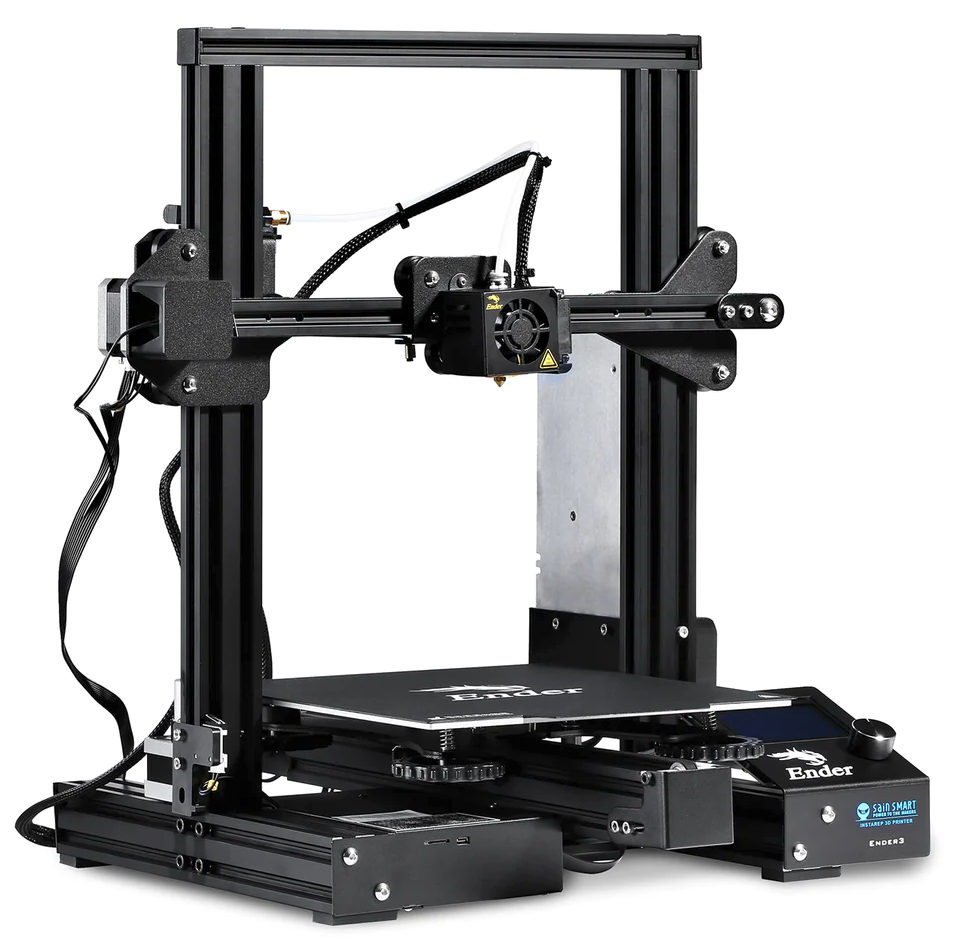
\includegraphics[width=.9\linewidth]{img/ender3.png}
\end{center}

% ==============================================================================
\pagebreak
\tableofcontents

% ==============================================================================
\pagebreak
\pagenumbering{arabic}  
\section{Introduction}
\label{sec:org82a736d}
The \href{https://www.creality.com/products/creality-ender-3-s1-pro-fdm-3d-printer}{Ender-3 S1 Pro printer from Creality} is an additive manufacturing device capable of printing using various types of polymer
materials.

\subsection{Practice: Benchy}
\label{sec:orgaa28782}
Throughout this guide, the practical parts will be demonstrated using a model name "Benchy" in the 3D printing
community.

\begin{center}
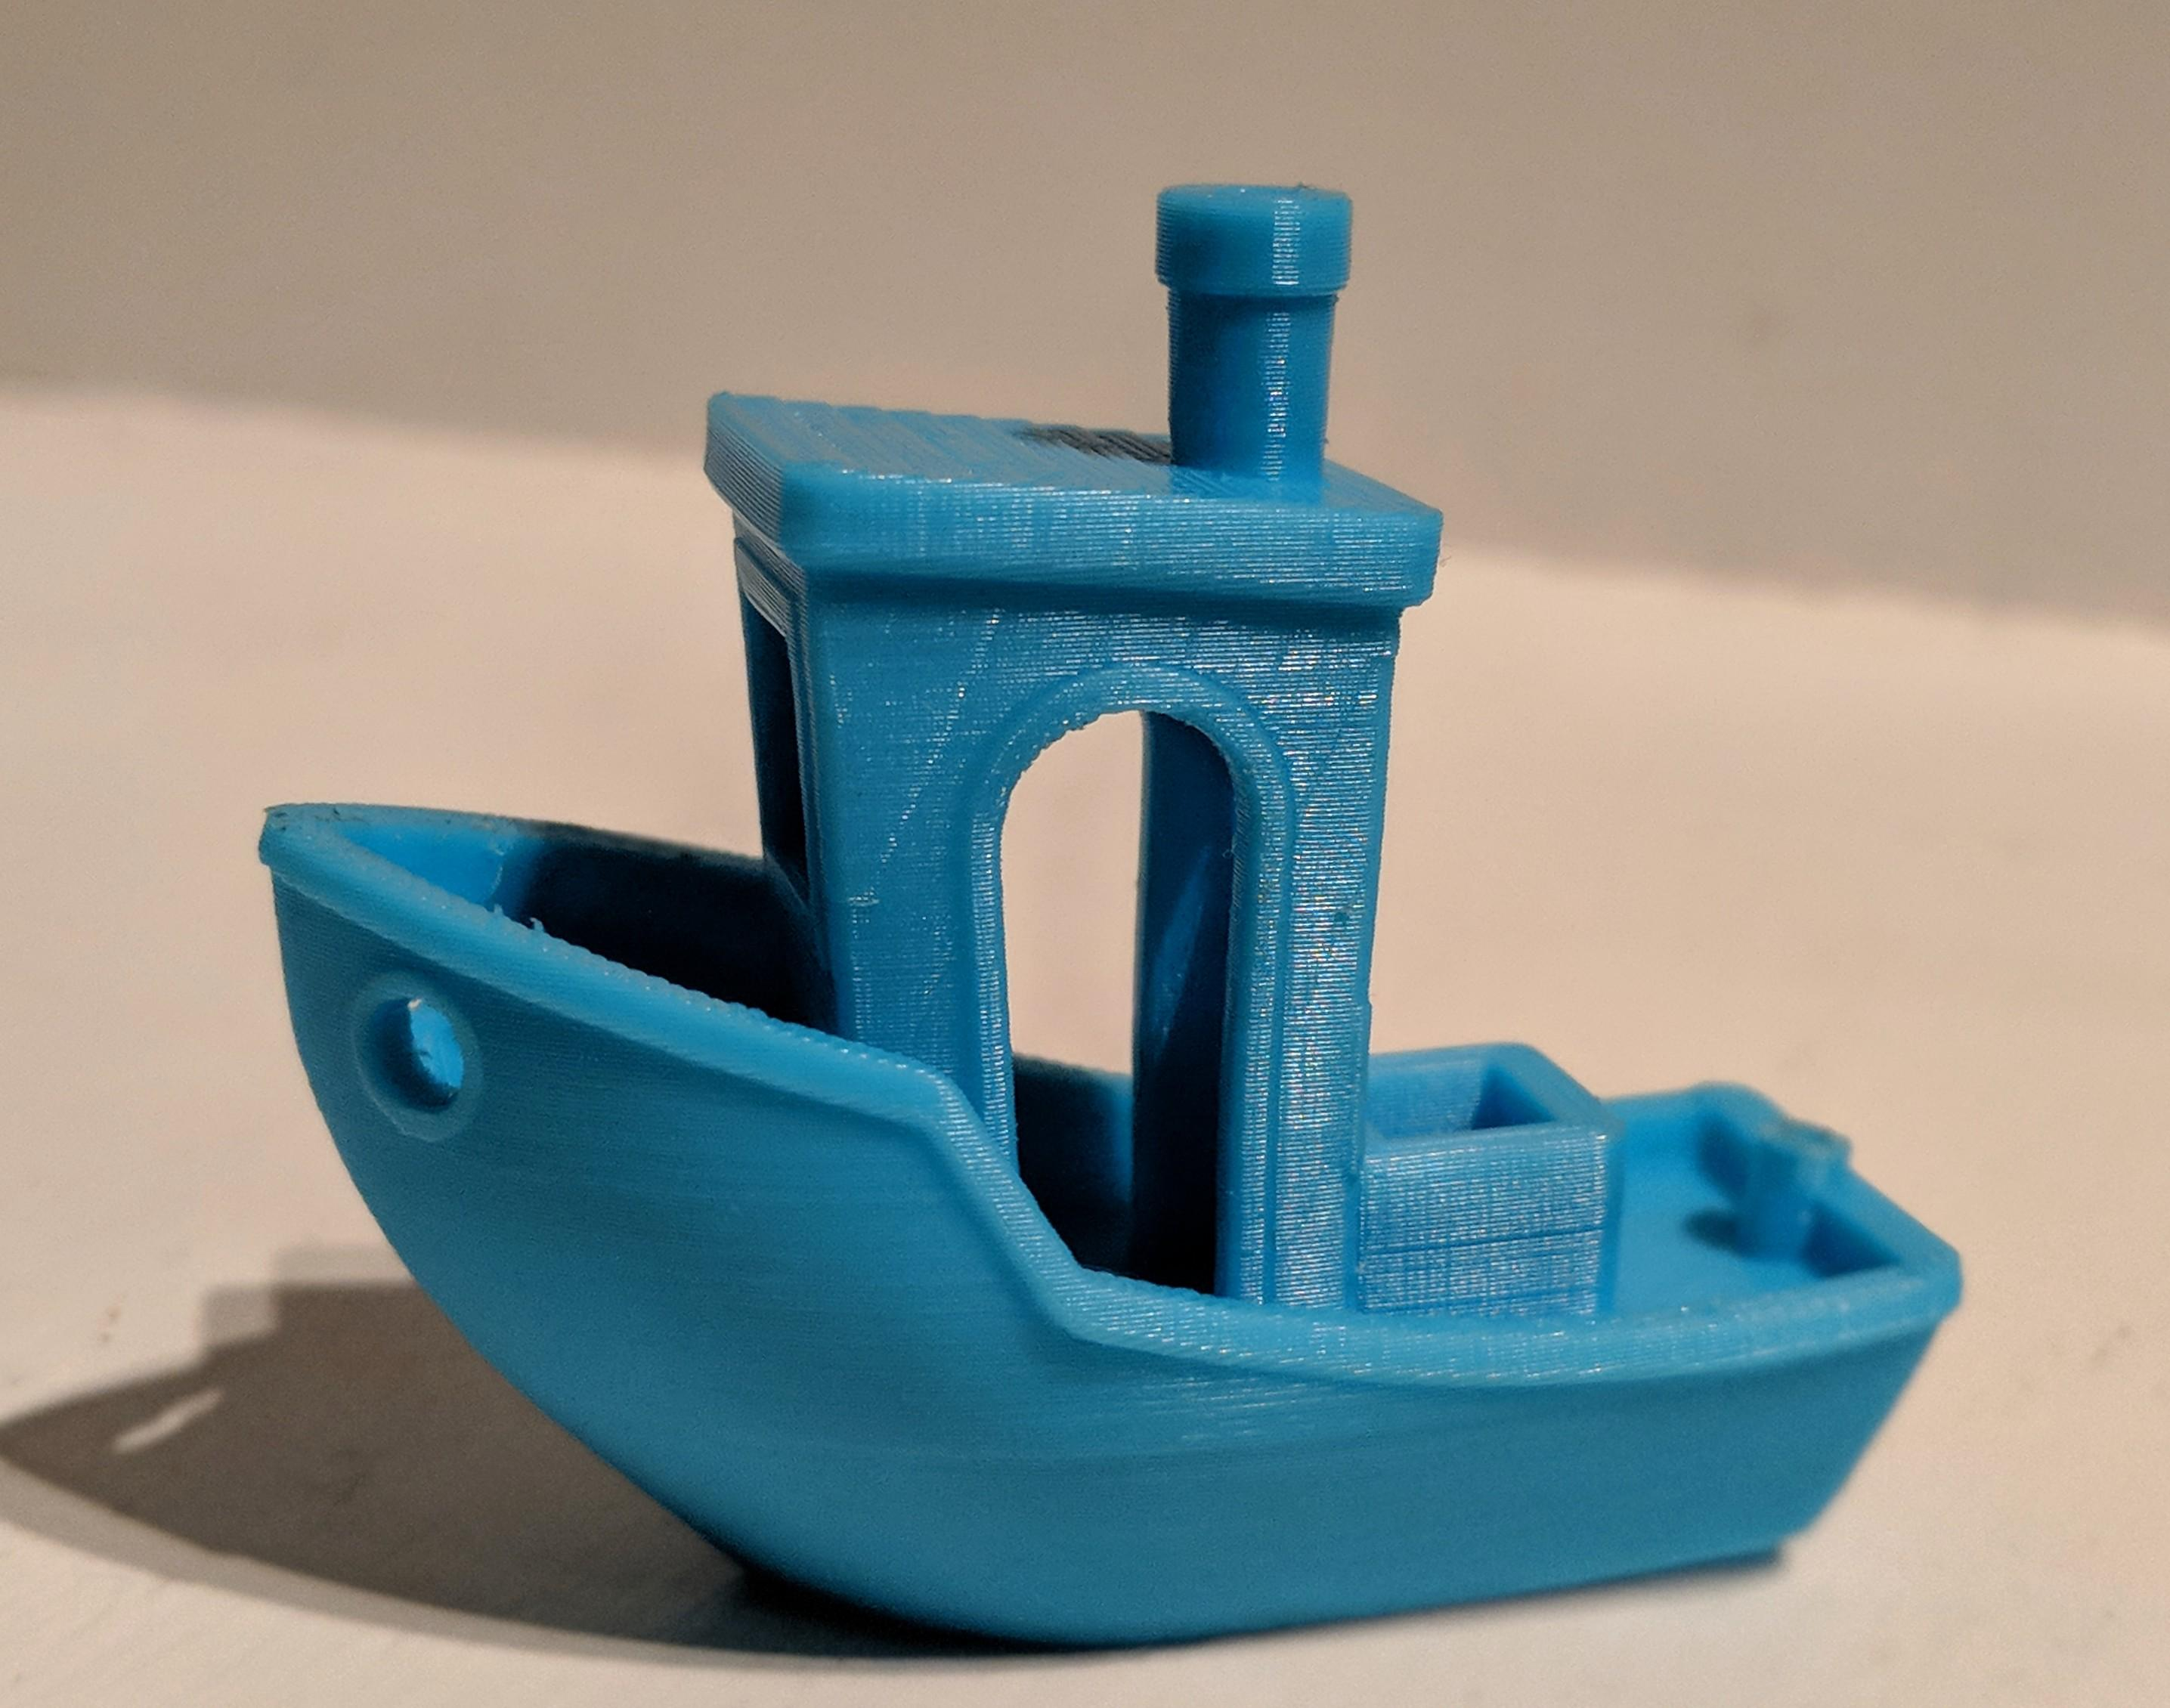
\includegraphics[width=.9\linewidth]{img/benchy.jpg}
\end{center}

This jolly boat has been used as a benchmark, stress test and calibration tool for printers for years. It has several
points in it's favor:
\begin{itemize}
\item The small base allows to test bed adhesion
\item The cabin part allows to test arches, bridges and small details
\item The hull allows to test overhang and see printing smoothness defects
\item The print is small and cute, and you want to make more of them!

The STL file can be found in many places, but I suggest getting it from \href{https://www.thingiverse.com/thing:763622/files}{the Thingiverse page},
where it can be downloaded without an account.
Note that many files are available; but you should get the one named "3DBenchy.stl",
since the other one are specials for multi-material printing.
\end{itemize}

% ==============================================================================
\section{Slicing}
\label{sec:org1941b78}
When a 3D model has been created or retrieved, it is needed to "slice" it in order for the file to become
understandable by the printer.

The slicing process takes a 3D model (typically in STL format) as an input, and creates a list of coordinates that directly represents
the path the printer head will follow to draw the part. Some other information are including, such as the printer head
speed or the printer temperature settings.

\subsection{Practice: Slicing Benchy using the Cura slicer}
\label{sec:orgf5fa04d}
It is possible to slice 3D models with a variety of tools, but in this guide, I choose to use
\href{https://ultimaker.com/software/ultimaker-cura/}{Ultimaker's Cura}. Even if primarily targeted at Ultimate's own printers, a number of
pre-sets for other machines are available, including our Ender-3.
The tool is also available for many platform, including Linux.

After installing the program, you will be greeted by a menu asking you to add a printer.
As visible in the next picture, you can choose "non-ultimaker".

\begin{center}
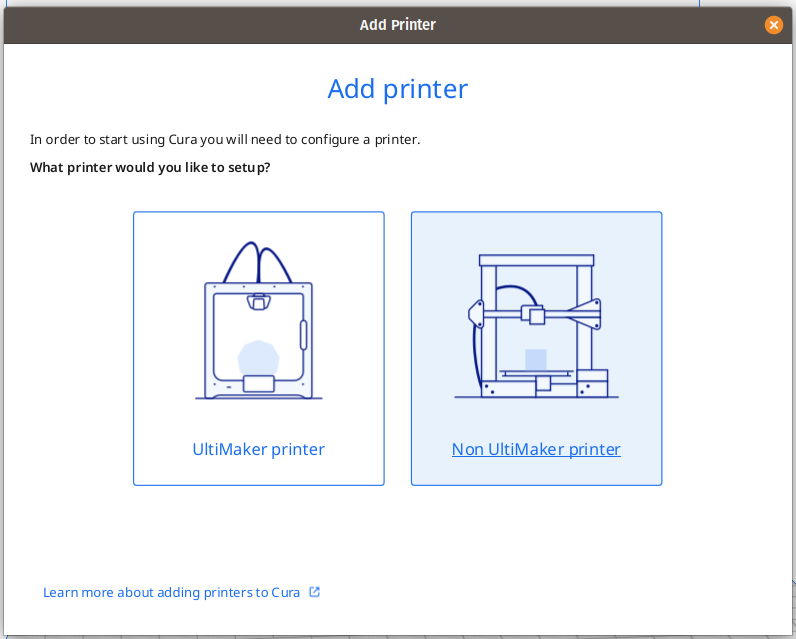
\includegraphics[width=.9\linewidth]{img/cura/1.png}
\end{center}

Then in the "non-network" list, you can find the model, in our case, Creality's Ender-3 S1 Pro.

\begin{center}
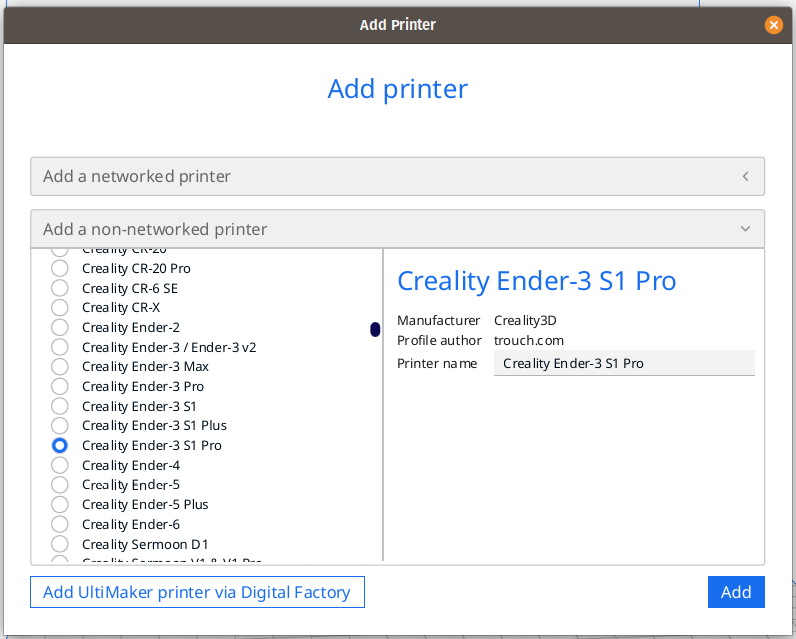
\includegraphics[width=.95\linewidth]{img/cura/2.png}
\end{center}

Upon validation, you will then arrive in the main view of the Cura software, as visible below.

\begin{center}
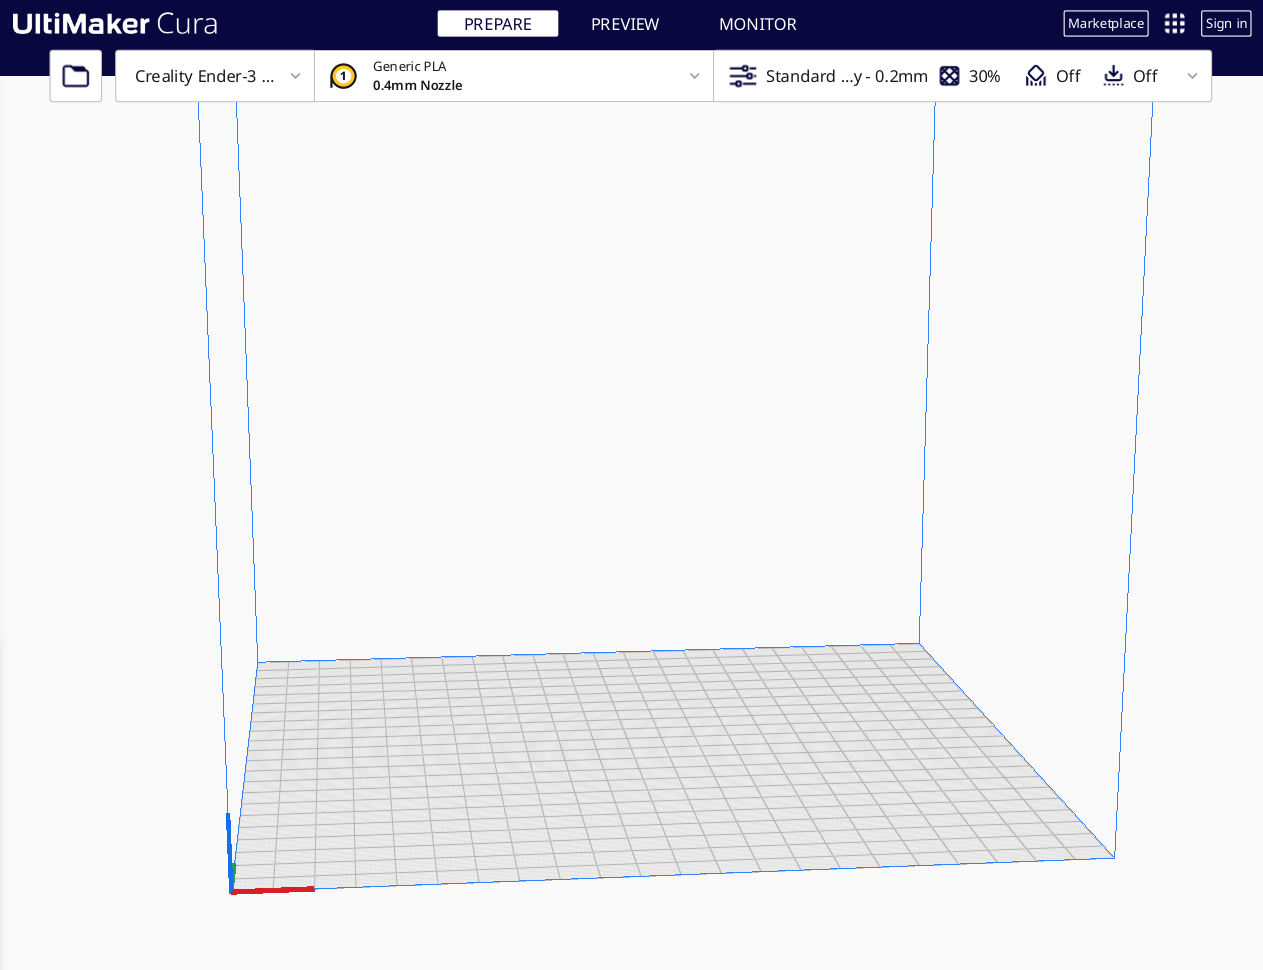
\includegraphics[width=.95\linewidth]{img/cura/3.png}
\end{center}

`From there', we have three tasks to do:
\begin{itemize}
\item Choosing the material
\item Choosing the printing settings
\item Importing the 3D model
\end{itemize}


For the material, the default one has temperature a little bit too low.
In that case, we will import a setting that was created to work well with the
ABS spool available.
The file can be downloaded \href{https://gitlab.com/sunoc/Marlin/-/snippets/2540628}{here}.

In the middle menu bar, you can click on the "Material" rolling menu, then scrolling down
and selecting "Manage Materials\ldots{}"

\begin{center}
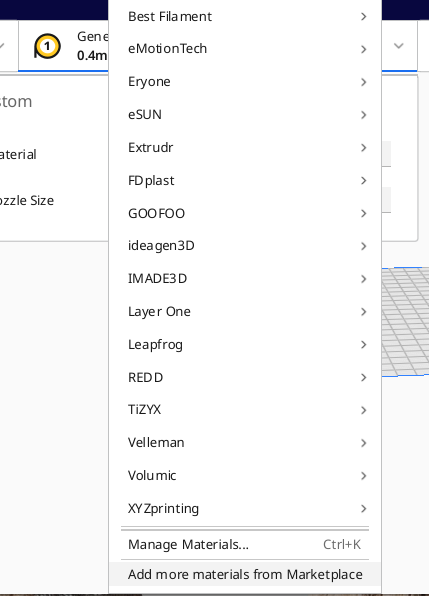
\includegraphics[width=.7\linewidth]{img/cura/4.png}
\end{center}

In the new window, one can simply click the "Import" button on the top right of the window,
and select the downloaded setting file.

\begin{center}
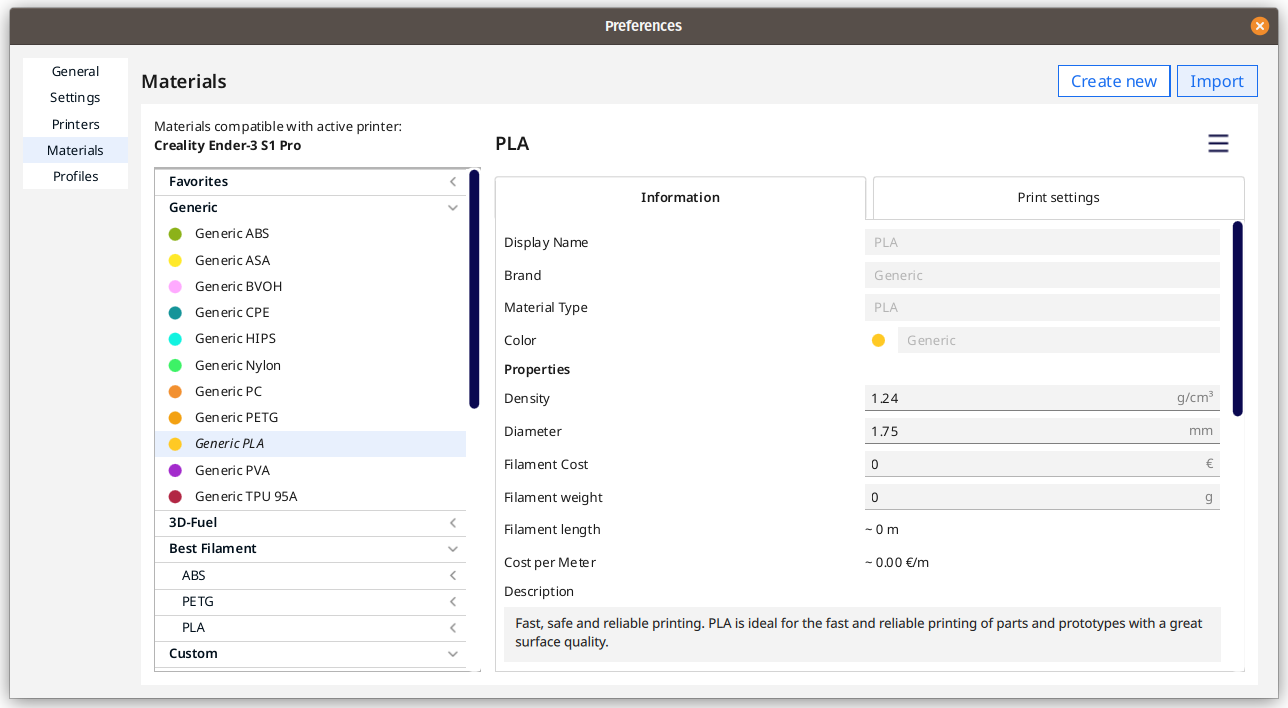
\includegraphics[width=.9\linewidth]{img/cura/5.png}
\end{center}

The new setting can now be chosen from the main view as the printing material.
It will be shown as "Kexcellent ABS", as visible below.

\begin{center}
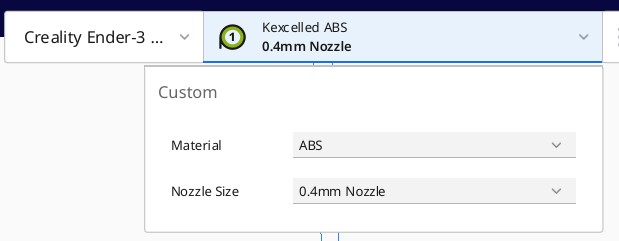
\includegraphics[width=.9\linewidth]{img/cura/6.png}
\end{center}

Now we have the material, we can focus on the settings.
On the next picture as well as on the right of you main frame menu, one
can see the default printing settings.

\begin{center}
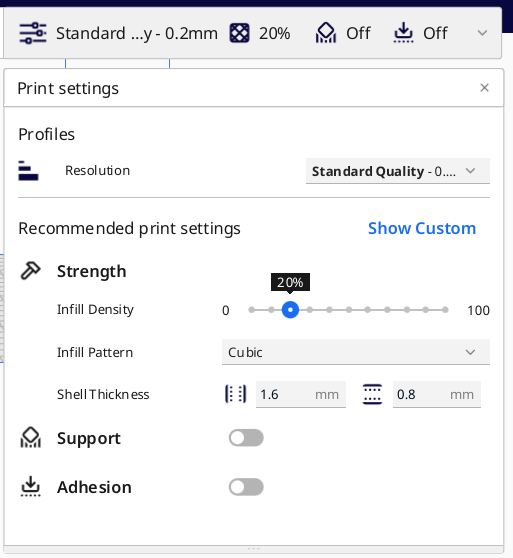
\includegraphics[width=.9\linewidth]{img/cura/7.png}
\end{center}

These are fine in general, but here are some tweaks I like to apply:
\begin{itemize}
\item Infill density of 30\%
\item Hexagonal infill pattern
\item Thicker, 2mm "walls"

These can be seen in the next picture.
\end{itemize}

\begin{center}
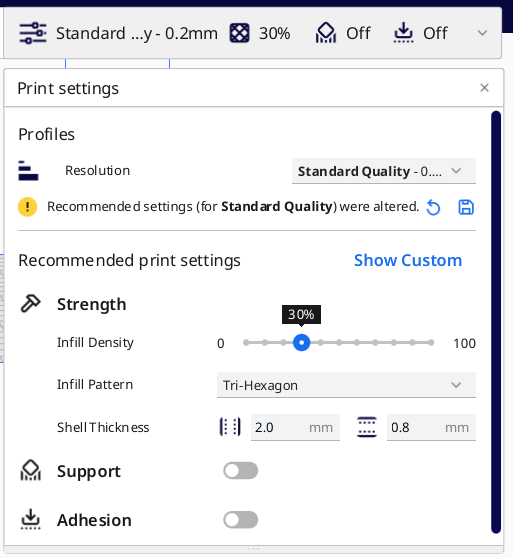
\includegraphics[width=.7\linewidth]{img/cura/8.png}
\end{center}

Finally, using the top left "directory" button, it is possible to import our benchy STL file, previously
downloaded from \href{https://www.thingiverse.com/thing:763622/files}{Thingiverse}.

When it's done, you should be seeing our tiny friend on your main Cura window, as follow:

\begin{center}
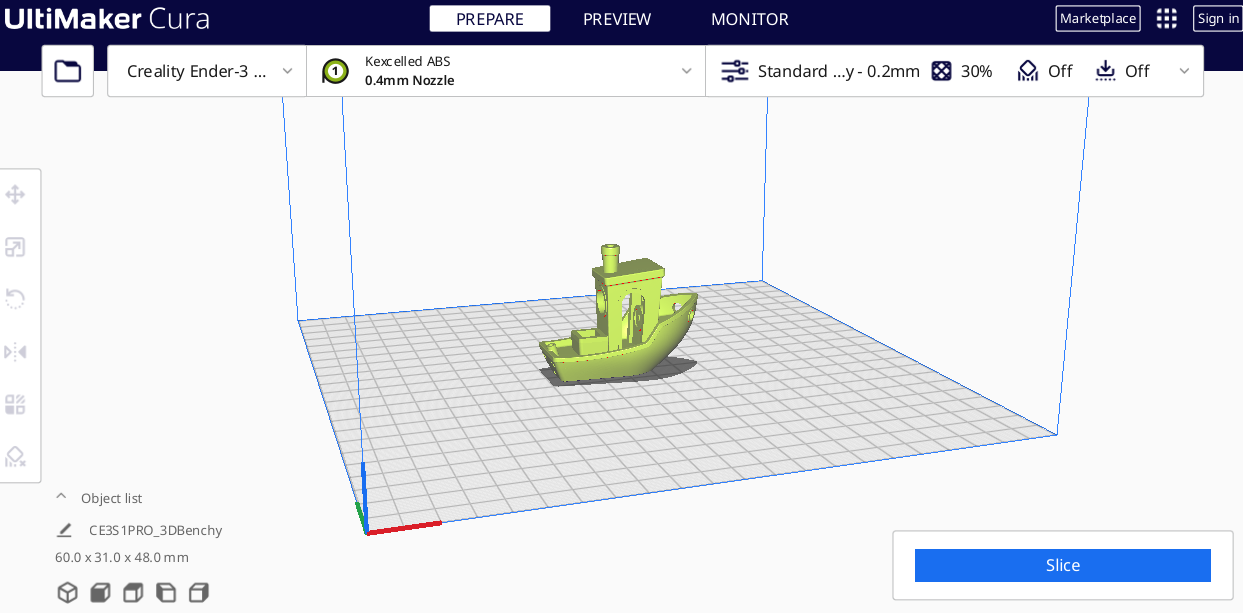
\includegraphics[width=1\linewidth]{img/cura/9.png}
\end{center}

Clicking the bottom right button will then proceed to the actual slicing.
It is then possible to see the result in the "Preview" tab, accessible in the top-most menu bar.

\begin{center}
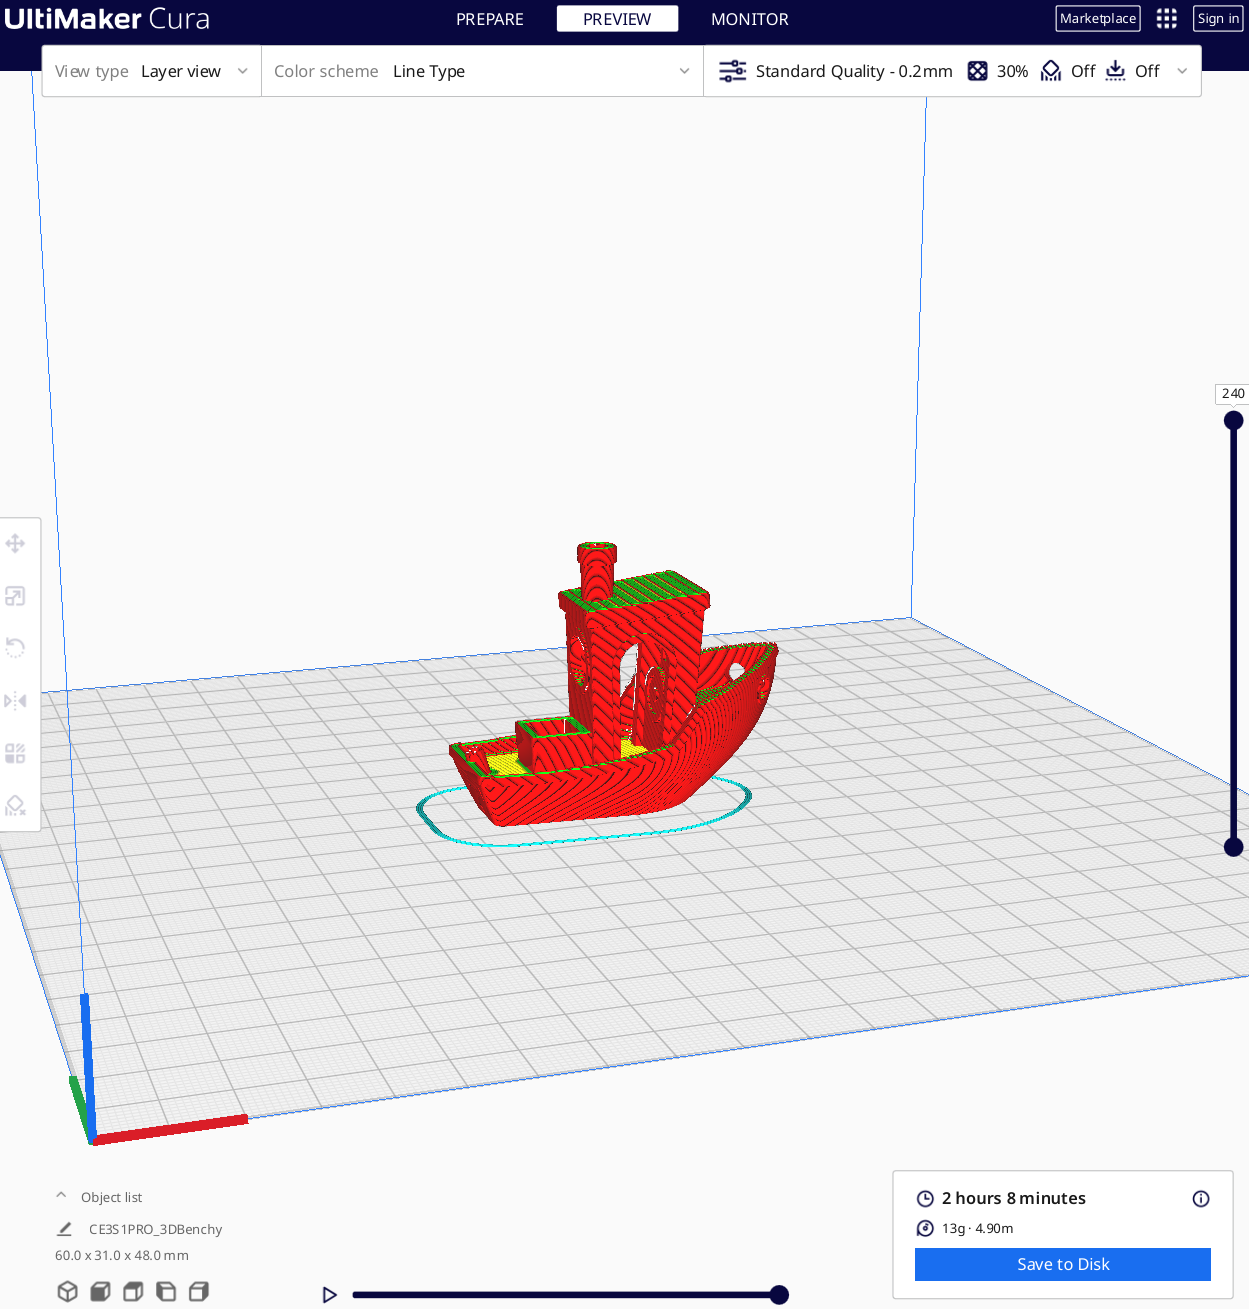
\includegraphics[width=.9\linewidth]{img/cura/10.png}
\end{center}

The New "Save" button on the bottom right of the window allows to save the result to the printers
SD card.

Once this is done, you are ready to print !



% ==============================================================================
\pagebreak
\section{Printing}
\label{sec:orge63f55d}

\subsection{Printers bed calibration}
\label{sec:org034d9ff}
Before starting using a new printer, it is important to calibrate the distance between the bed and the printing head.
Having a well calibrated bed helps for a variety of issues, from printing defects to bed adhesion.

For the Ender-3 printer, \href{https://img.staticdj.com/8f39f619af6bf34e5afb36ddbf2a0229.pdf?spm=..page\_1995605.download\_support\_1.1\&spm\_prev=..product\_5e45abfb-4541-4c92-ba93-cfba9a1e3ea4.nav\_link\_store\_1.1}{the reference manual}, pp. 6, presents the  way to use the auto-calibration.
This, however, doesn't seem to exactly cover all the cases, so I will present here how it was done in my case.

\begin{figure}[H]
    \centering 
    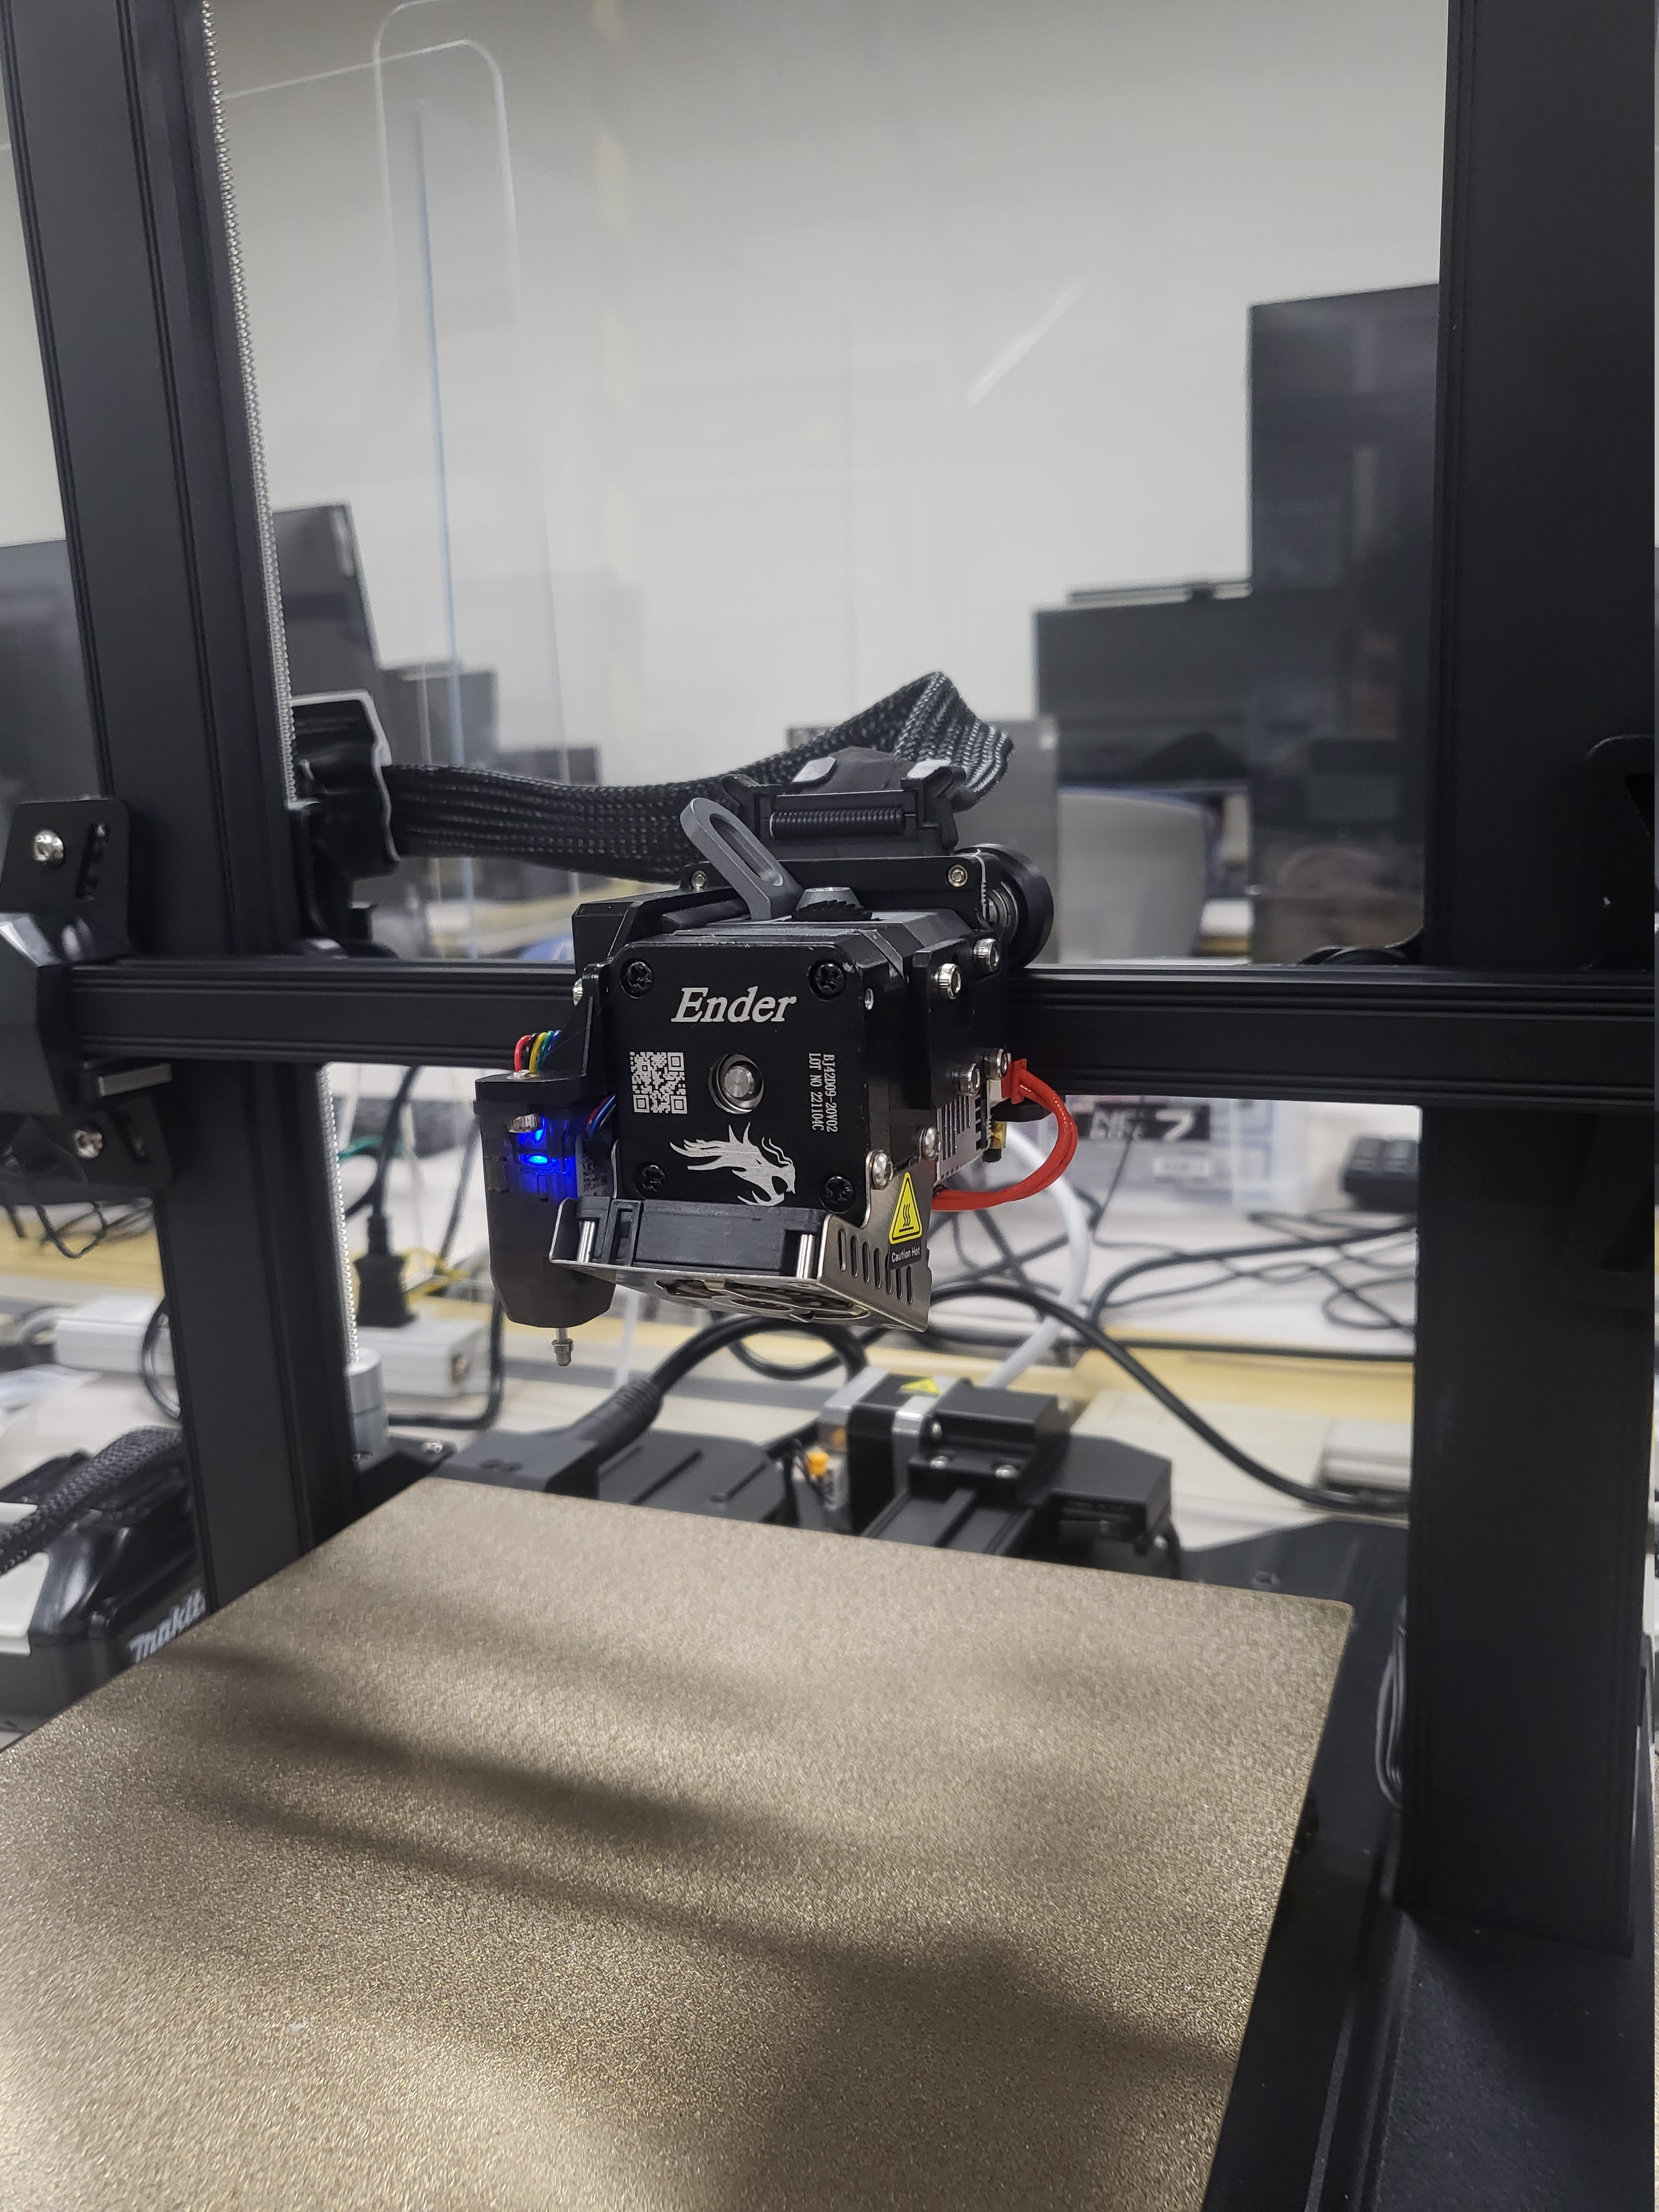
\includegraphics[width=0.8\textwidth]{img/ender/1.jpg} 
    \caption{We want to calibrate the distance between the printing head nozzle and the adhesion bed.}
    \label{fig:ender1}
\end{figure}
  
\begin{figure}[H]
    \centering 
    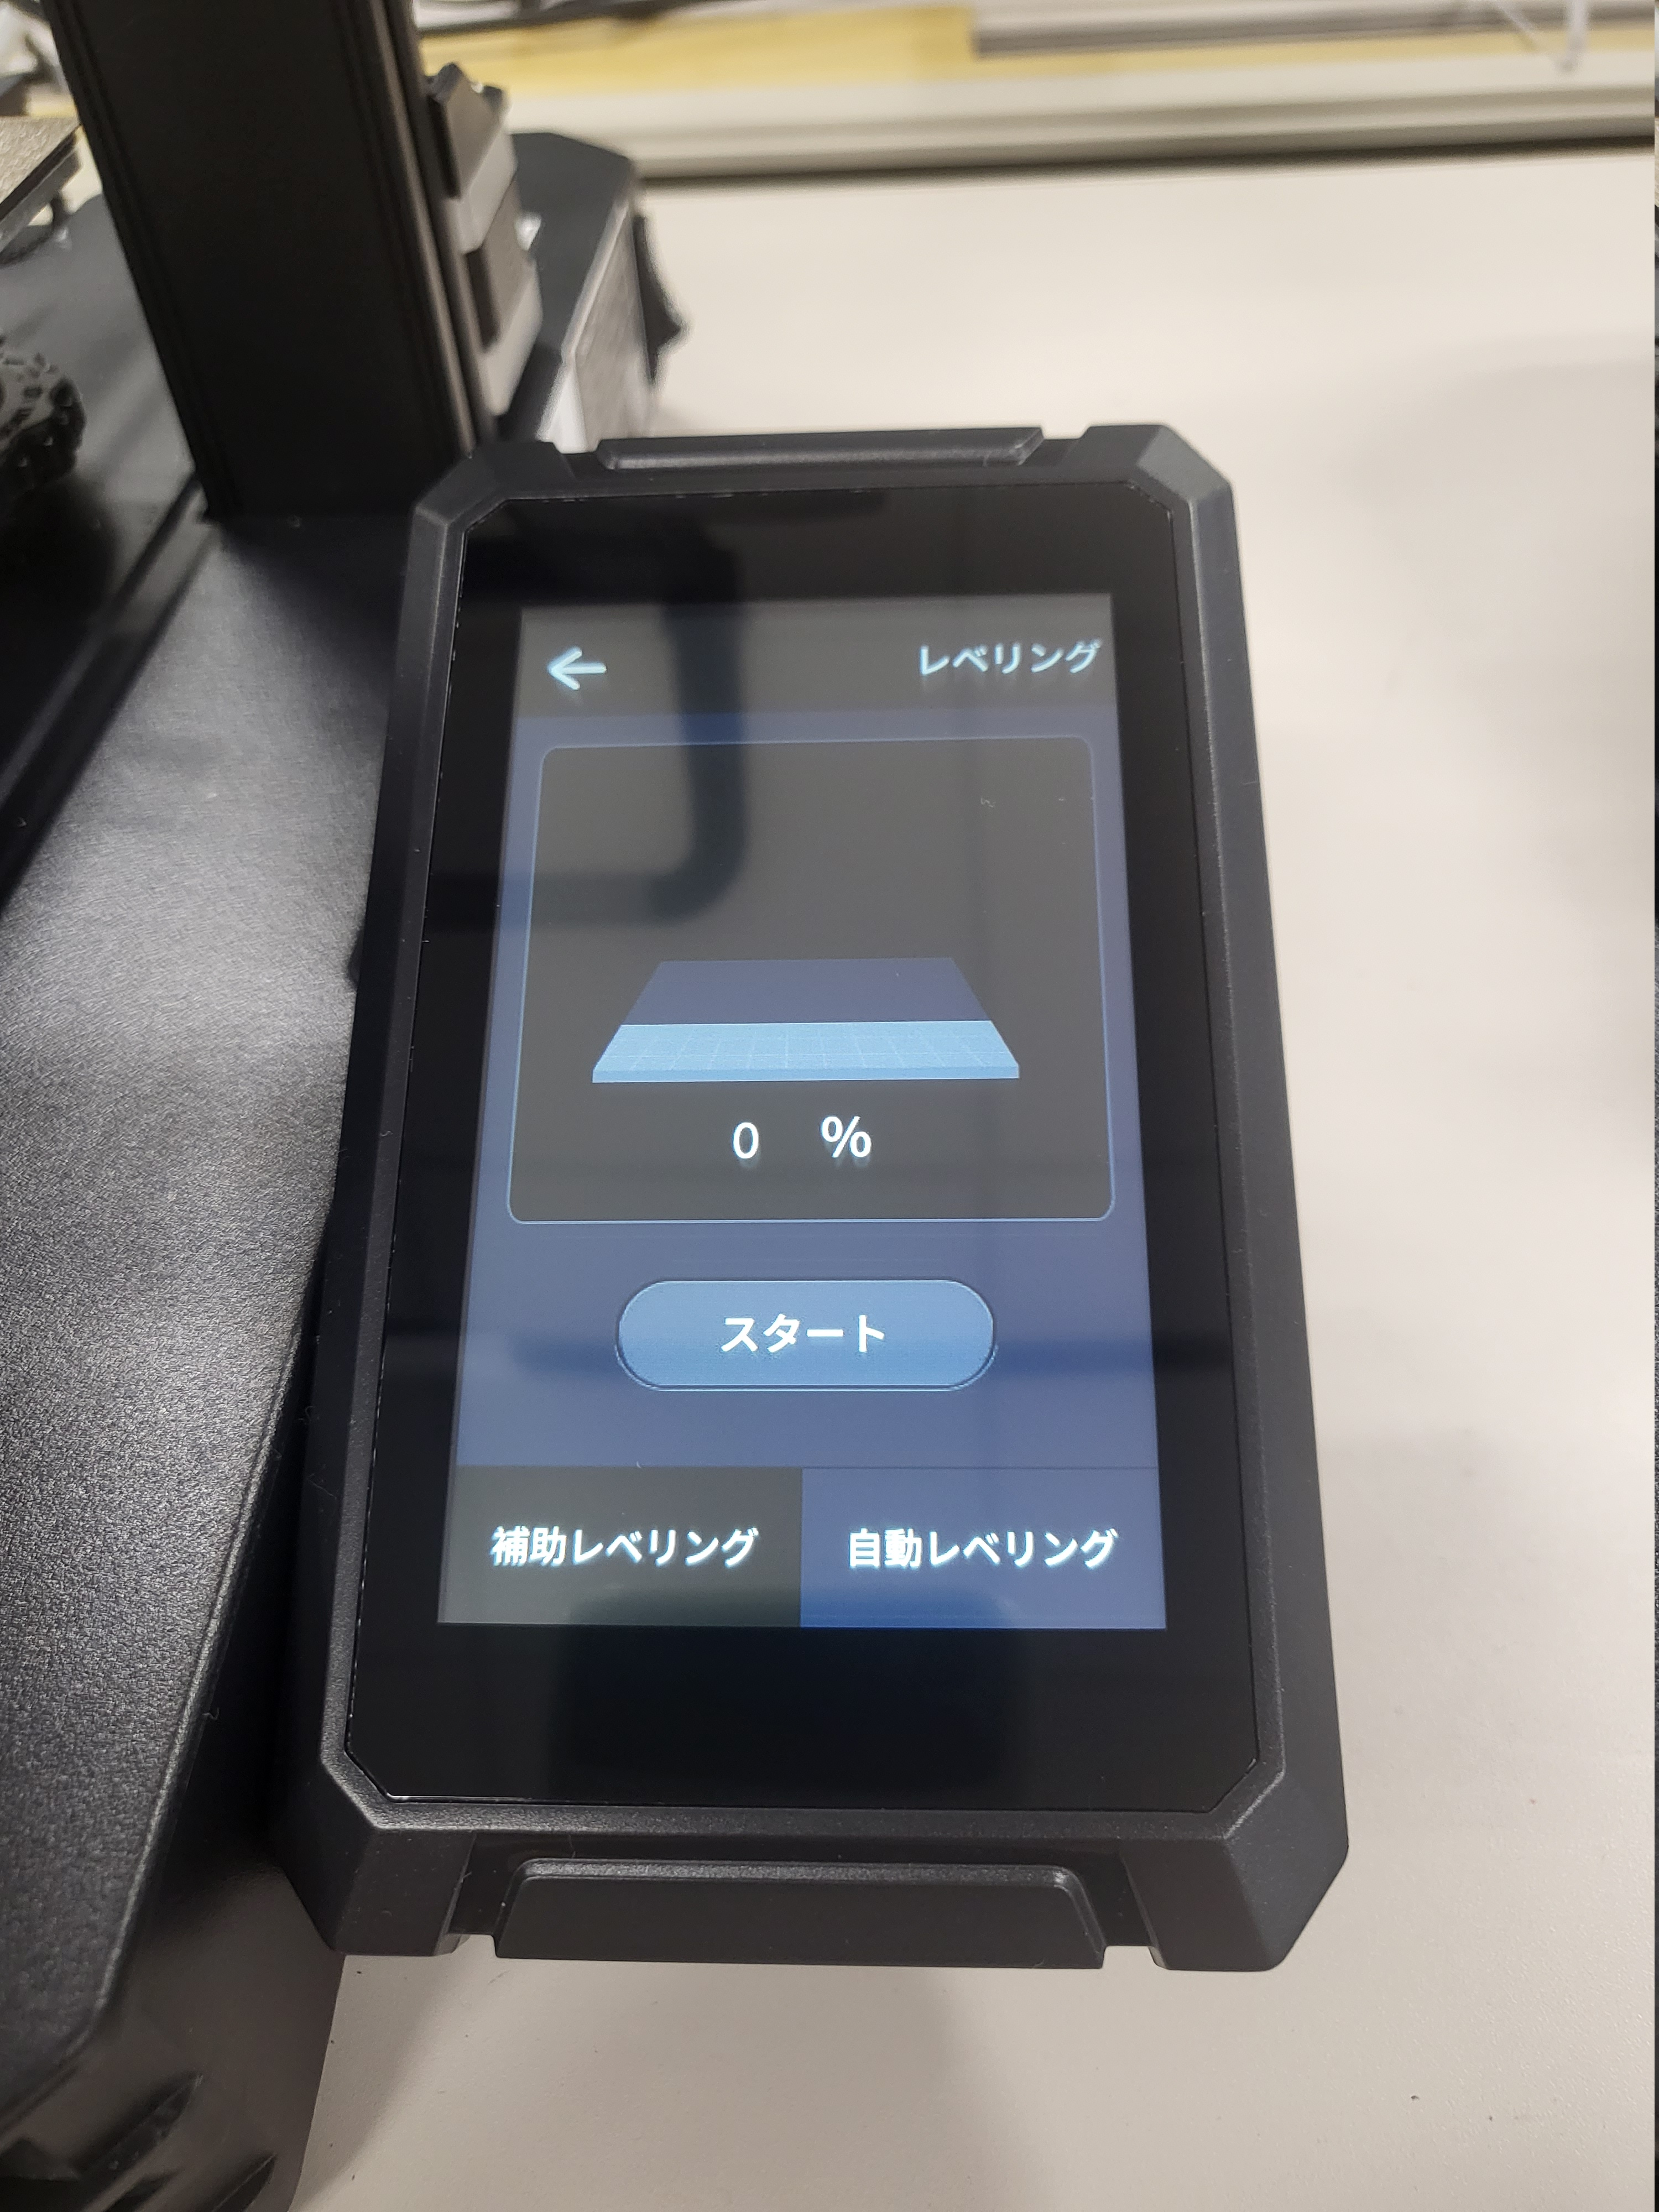
\includegraphics[width=0.6\textwidth]{img/ender/2.jpg} 
    \caption{In the settings, we can find this menu for starting the auto-calibration of the beds hight.}
    \label{fig:ender2}
\end{figure}

\begin{figure}[H]
    \centering 
    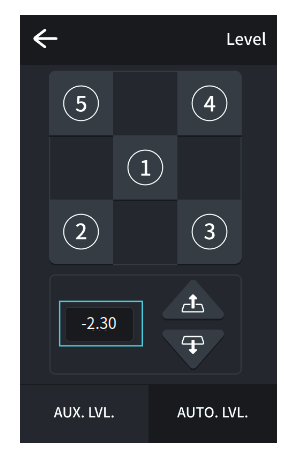
\includegraphics[width=0.3\textwidth]{img/ender/3.png} 
    \caption{From this menu, you can adjust the hight for the head with the arrow buttons for five zones of the bed. Proceed in numerical order.\\ \textit{Source:} \href{https://img.staticdj.com/8f39f619af6bf34e5afb36ddbf2a0229.pdf?spm=..page\_1995605.download\_support\_1.1\&spm\_prev=..product\_5e45abfb-4541-4c92-ba93-cfba9a1e3ea4.nav\_link\_store\_1.1}{the reference manual}}
    \label{fig:ender3}
\end{figure}

\begin{figure}[H]
    \centering 
    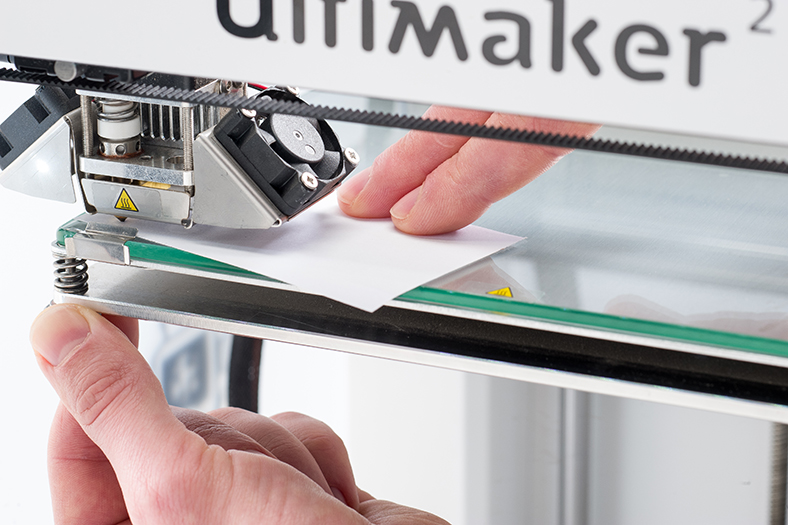
\includegraphics[width=0.4\textwidth]{img/ender/4.jpg} 
    \caption{It can be challenging to estimate the correct hight of the nozzle. A technic that works well is to slide a piece of paper between the nozzle and the bed. If you can still move the paper but feel some resistance, the distance is good.\\ 
    \textit{Source:} \href{https://blog.discoverthat.co.uk/2015/06/calibrate-3d-printer.html}{A blog about Ultimaker's printers}}
    \label{fig:ender4}
\end{figure}

\begin{figure}[H]
    \centering 
    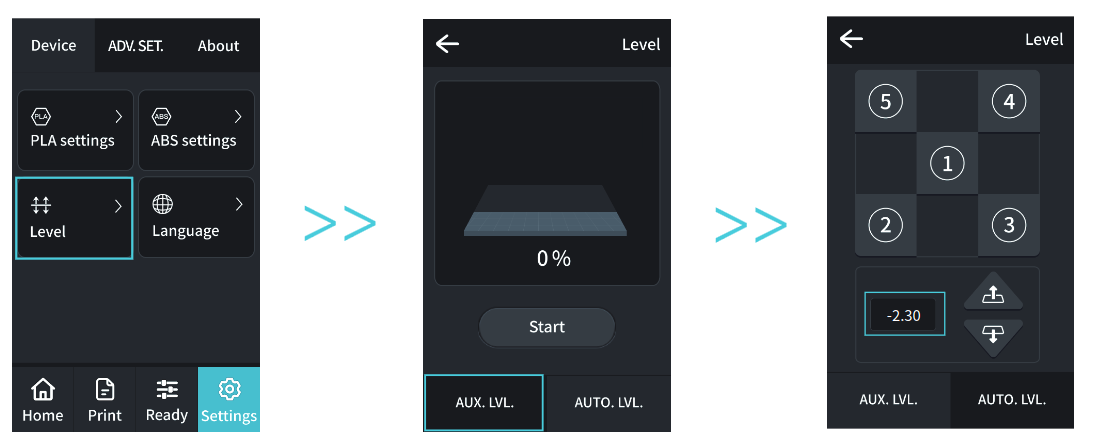
\includegraphics[width=0.8\textwidth]{img/ender/3a.png} 
    \caption{If more adjustement is needed, the following option allows to adjust the hight of the bed itself, for the same five areas.\\ 
    \textit{Source:} \href{https://img.staticdj.com/8f39f619af6bf34e5afb36ddbf2a0229.pdf?spm=..page\_1995605.download\_support\_1.1\&spm\_prev=..product\_5e45abfb-4541-4c92-ba93-cfba9a1e3ea4.nav\_link\_store\_1.1}{the reference manual}}
    \label{fig:ender3a}
\end{figure}

\begin{figure}[H]
    \centering 
    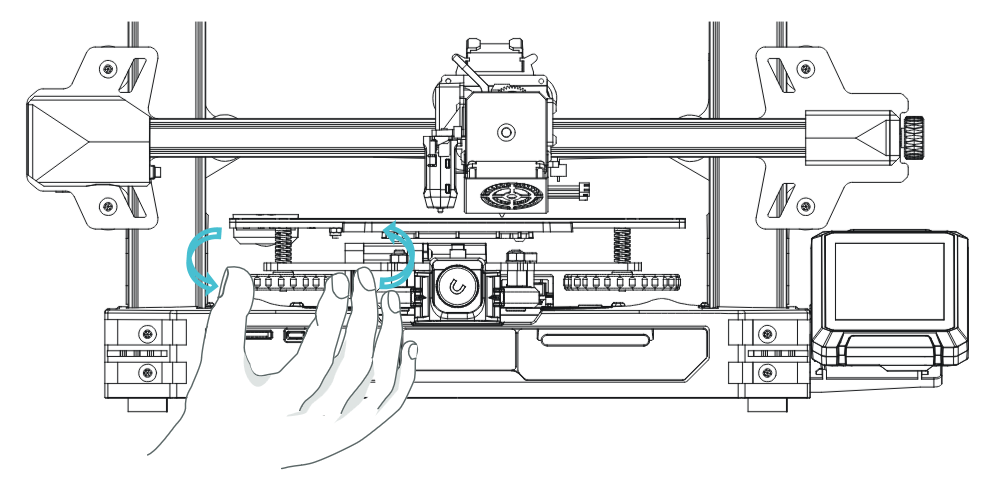
\includegraphics[width=0.8\textwidth]{img/ender/3b.png} 
    \caption{From this setting, it is possible to ajust the hight of the bed by using the scews and handles directly under the beg. Be carful to re-check all fives points multiple times after a large adjustement has been made.\\ 
    \textit{Source:} \href{https://img.staticdj.com/8f39f619af6bf34e5afb36ddbf2a0229.pdf?spm=..page\_1995605.download\_support\_1.1\&spm\_prev=..product\_5e45abfb-4541-4c92-ba93-cfba9a1e3ea4.nav\_link\_store\_1.1}{the reference manual}}
    \label{fig:ender3b}
\end{figure}


\subsection{Printers temperatures calibration, head pre-heating for filament insertion}
In the printer settings, it is possible to view and modify the temperature settings for the nozzle and of the printing beg of the Ender-3.

The goal is to set the desired settings in order to be able to load the filament.

\label{sec:org2c62615}
\begin{figure}[H]
    \centering 
    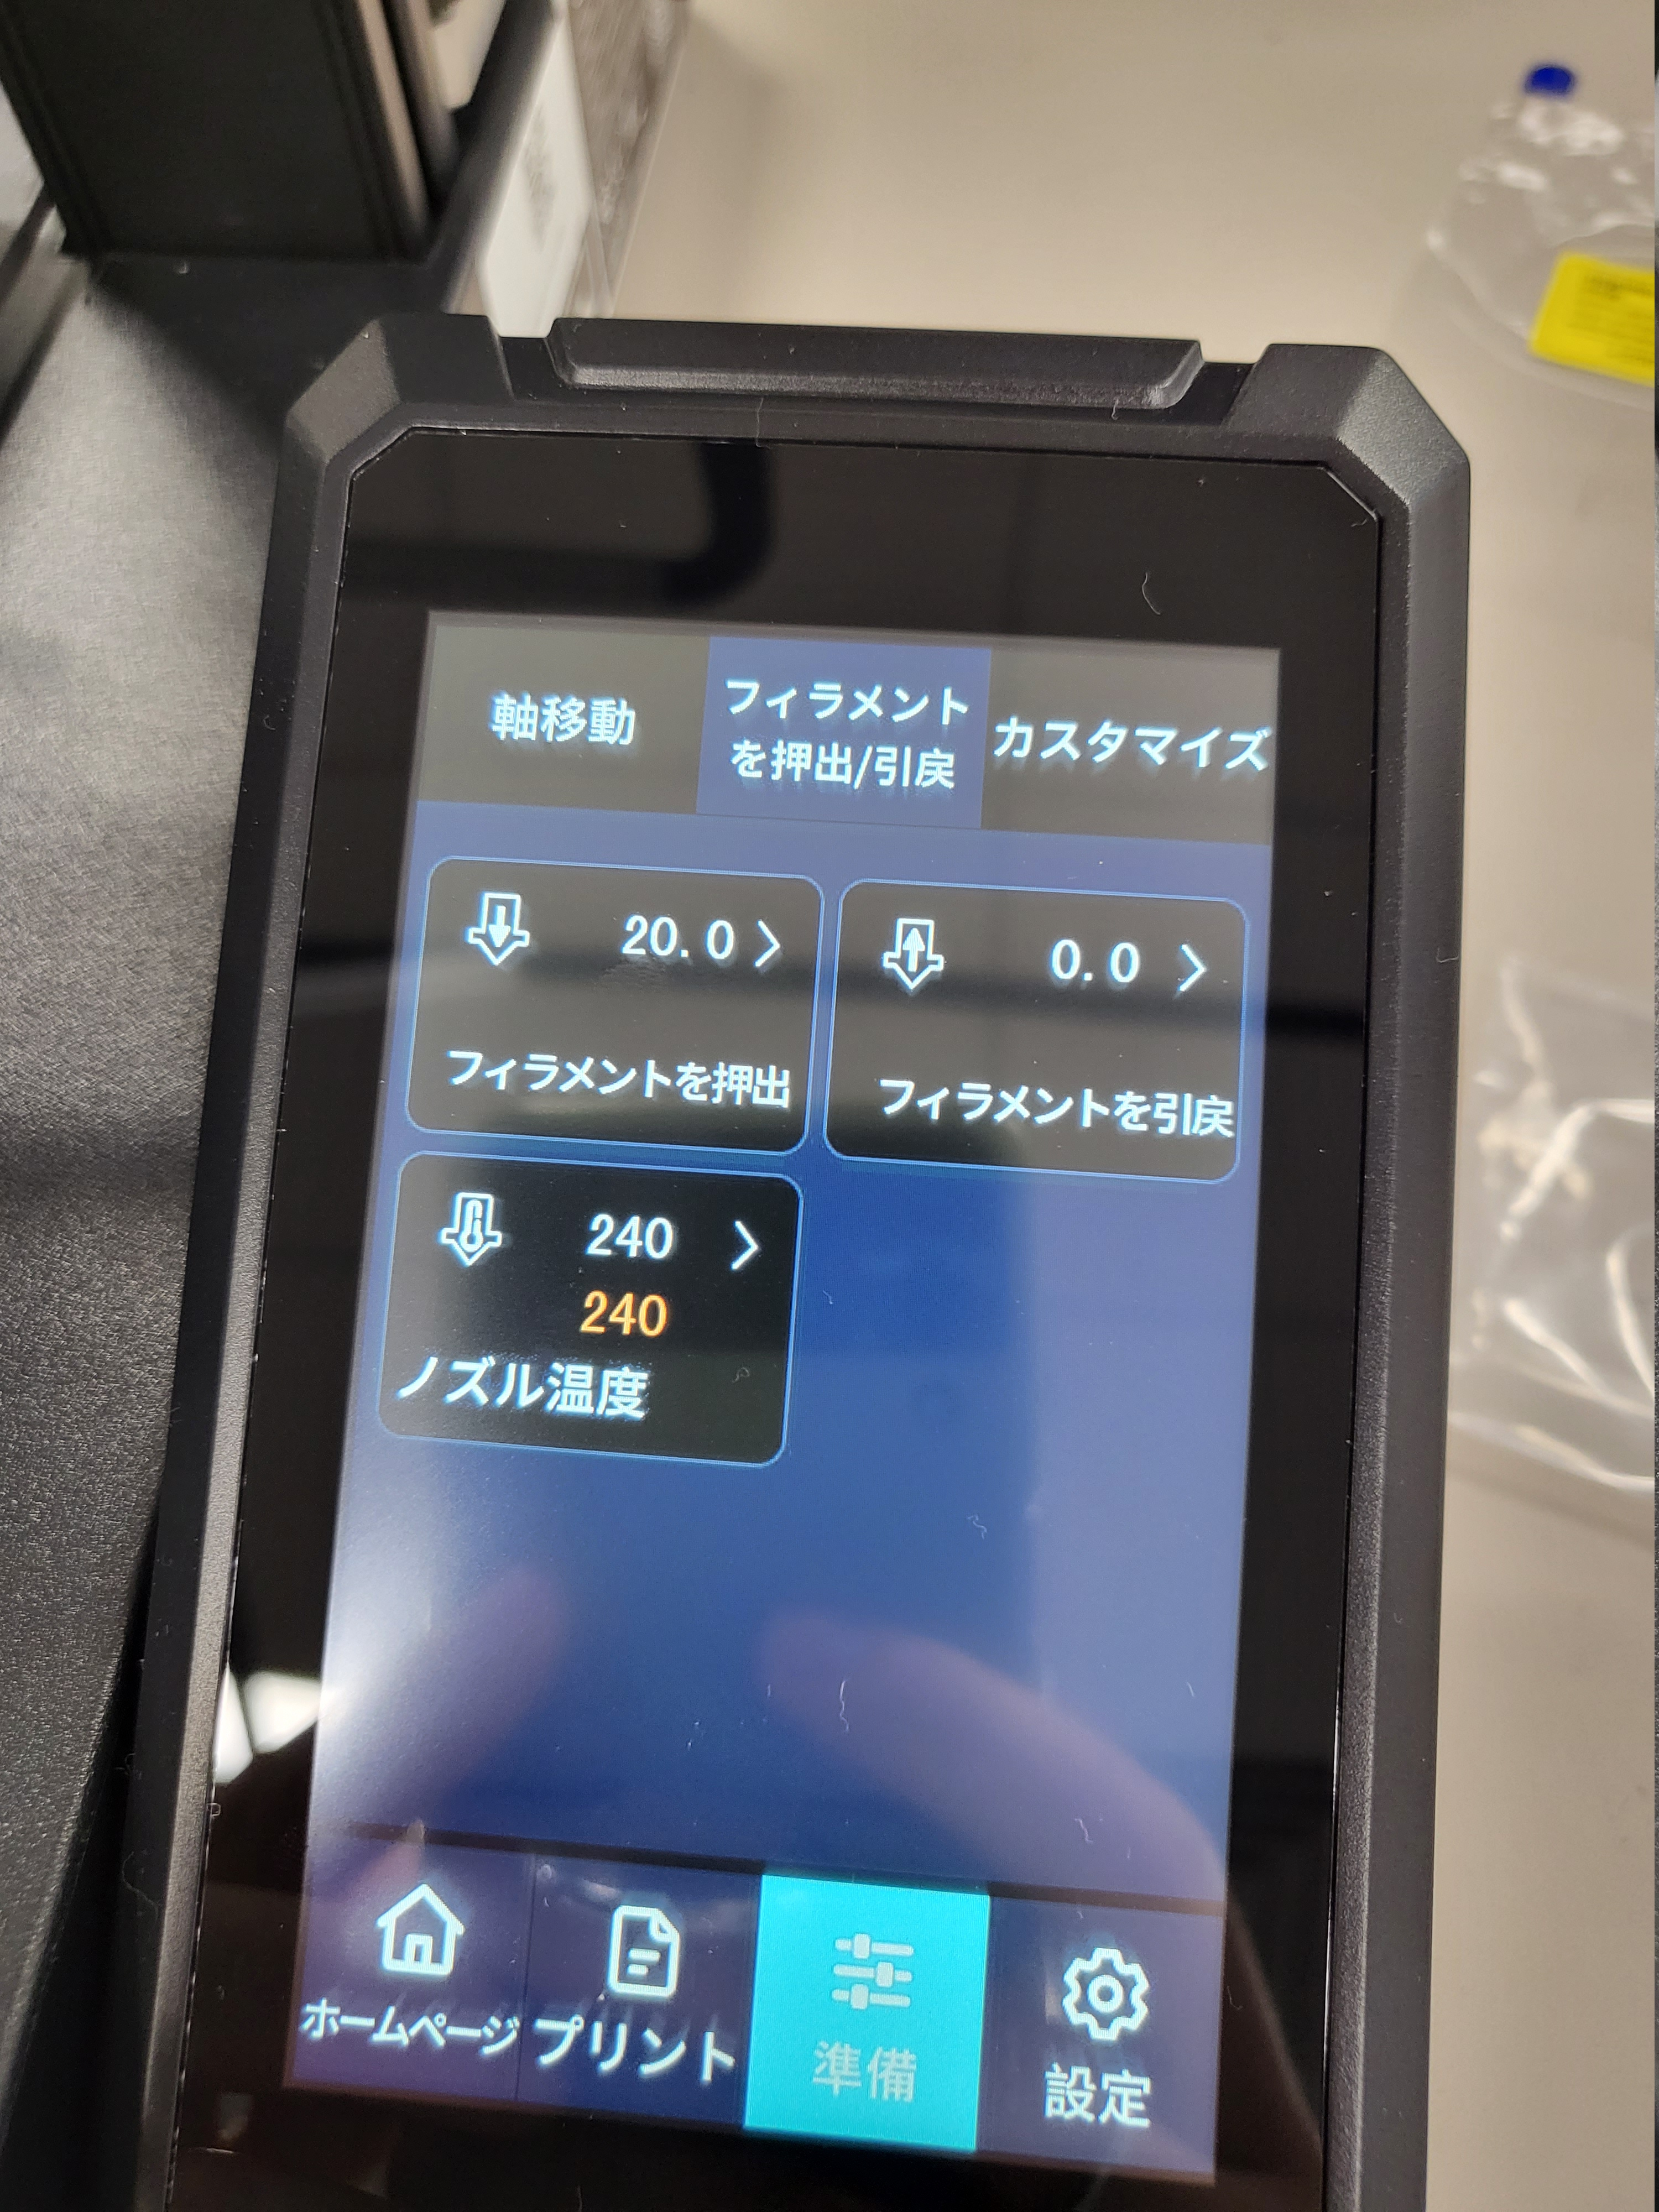
\includegraphics[width=0.4\textwidth]{img/ender/5.jpg} 
    \caption{The temperatures of the bed and nozzle are set in the material configuration when loading a model, and can be seen in this menu.}
    \label{fig:ender5}
\end{figure}

\begin{figure}[H]
    \centering 
    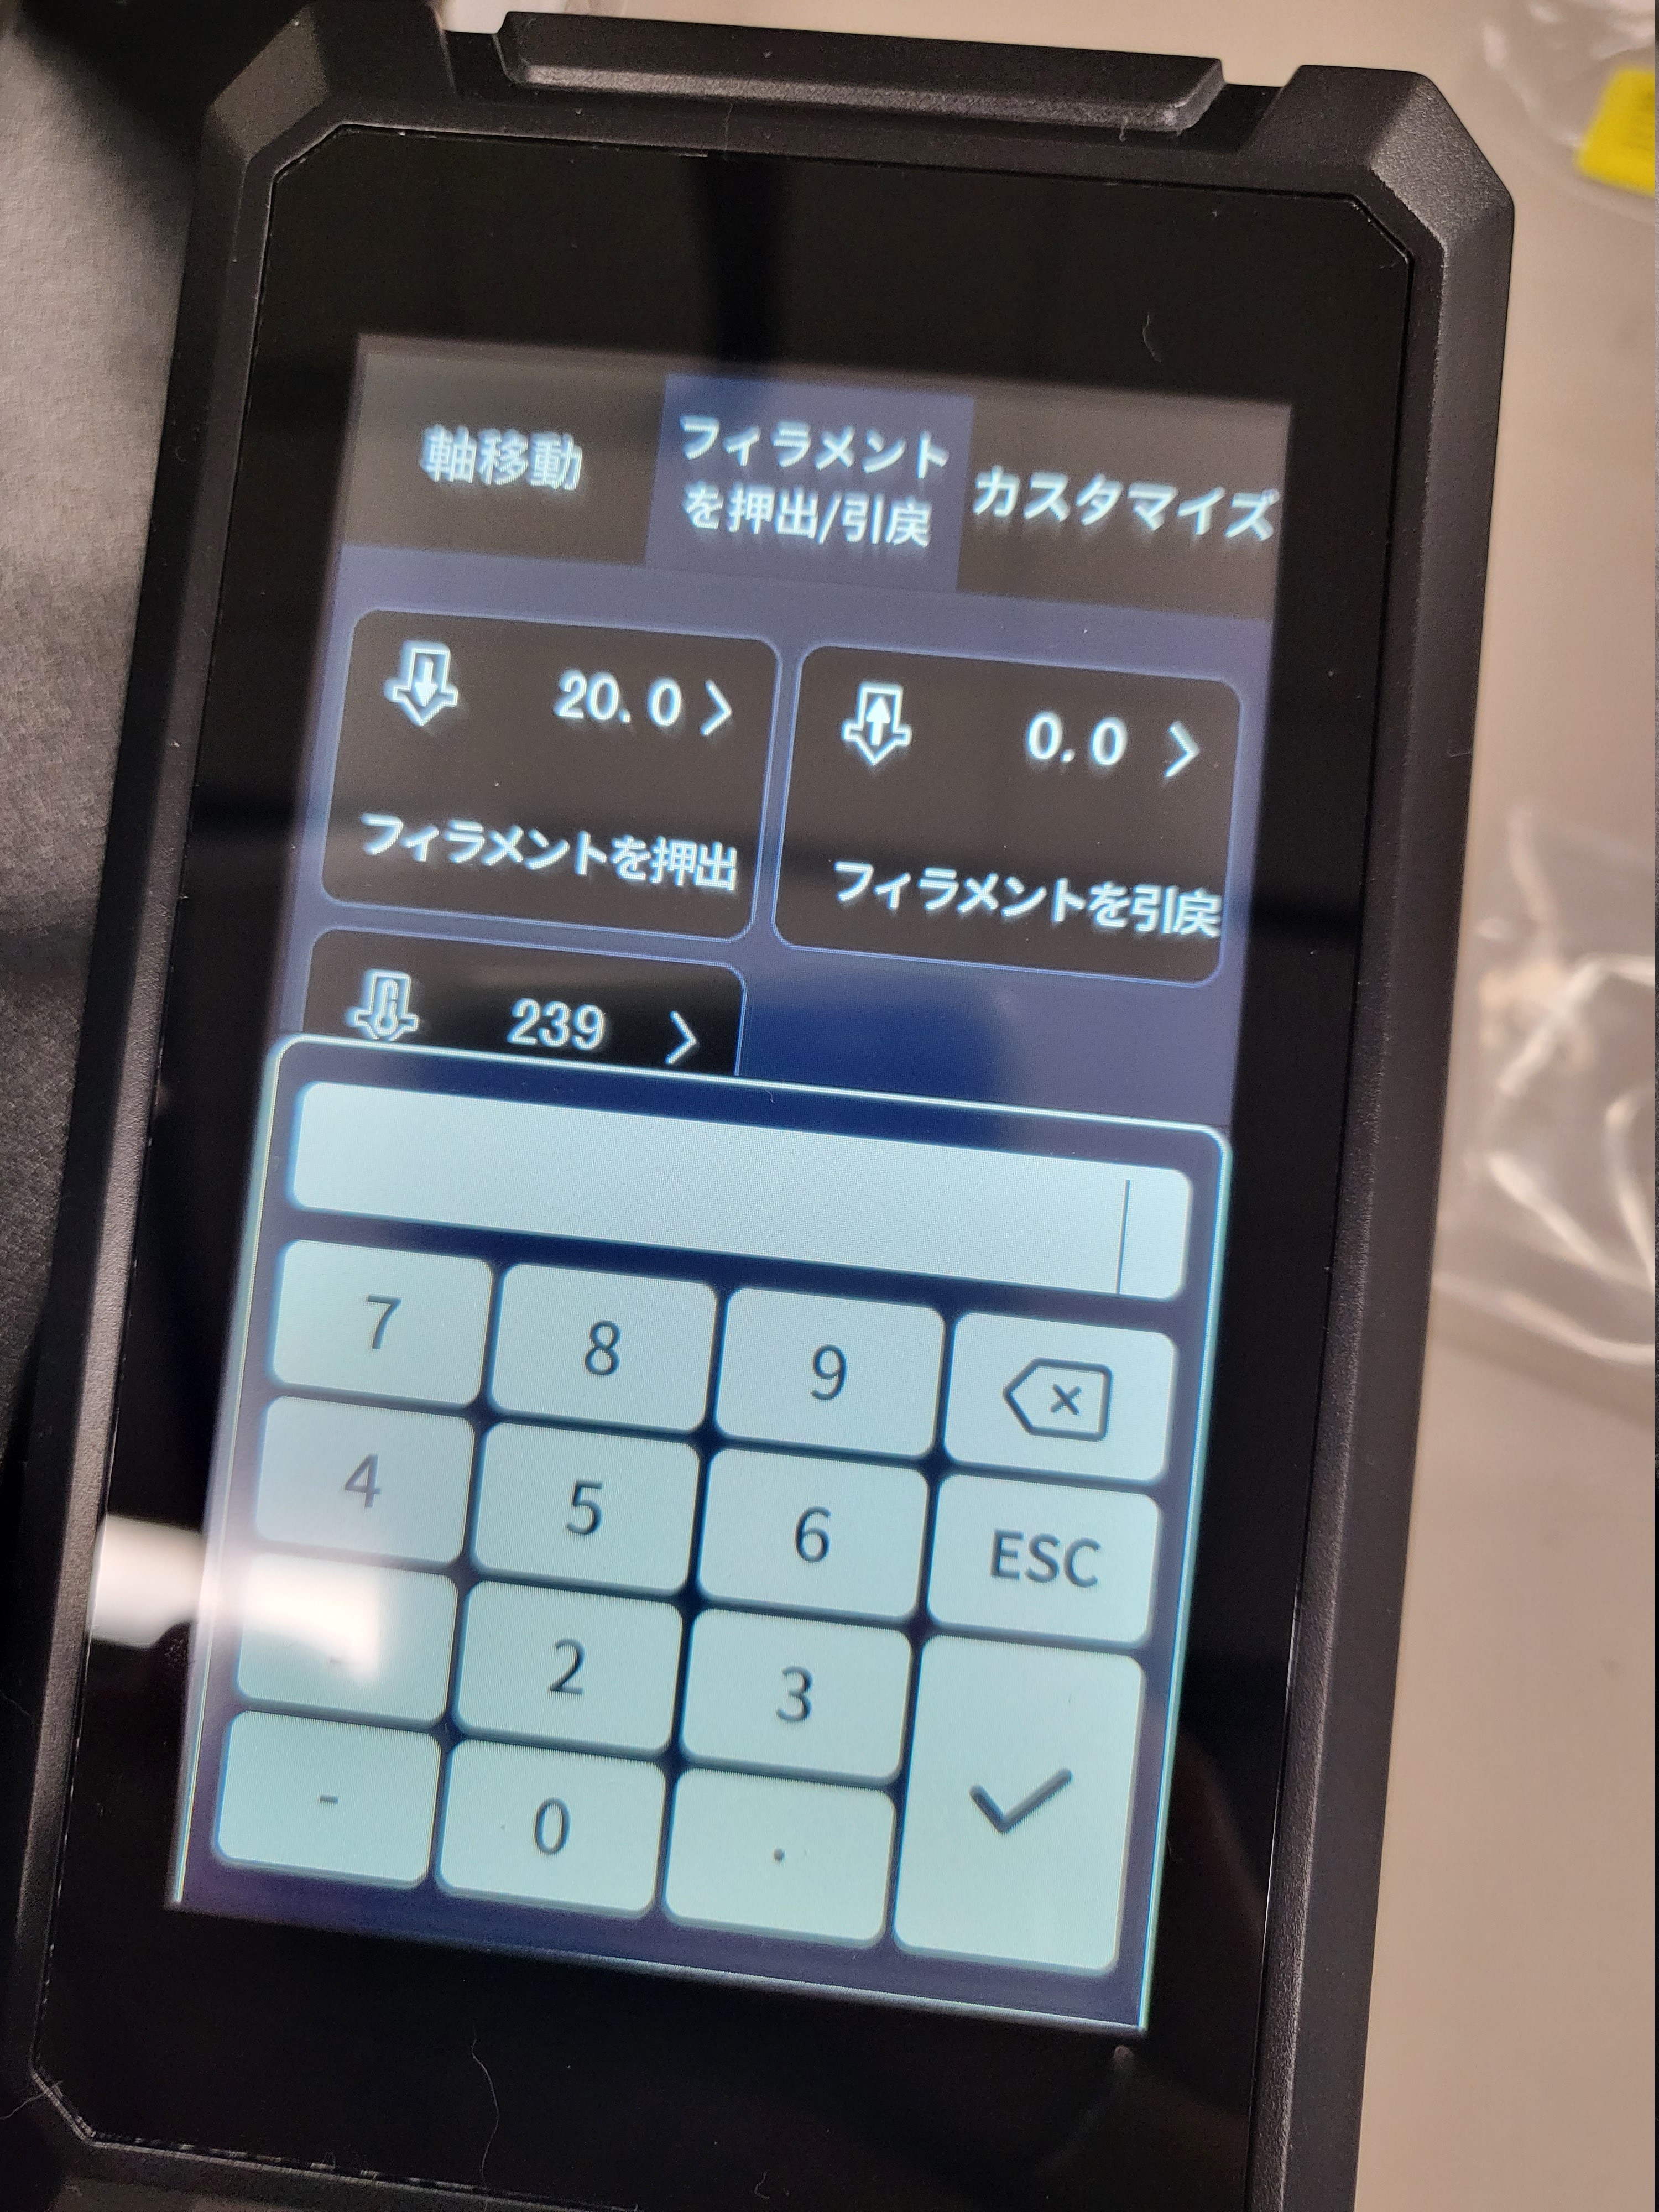
\includegraphics[width=0.4\textwidth]{img/ender/6.jpg} 
    \caption{It is possible to ajust them manually from the same menu, for example when perparing the printer in advance; or to make some temperatre adjustement test for a new material.}
    \label{fig:ender6}
\end{figure}


\subsubsection{Loading the filament}
Now we can set some temperature, it is possoble to load the printing head with a new filament. The nozzle should be around the printing temprature for the filament material to be soft enough to go through the nozzle.

\begin{figure}[H]
    \centering 
    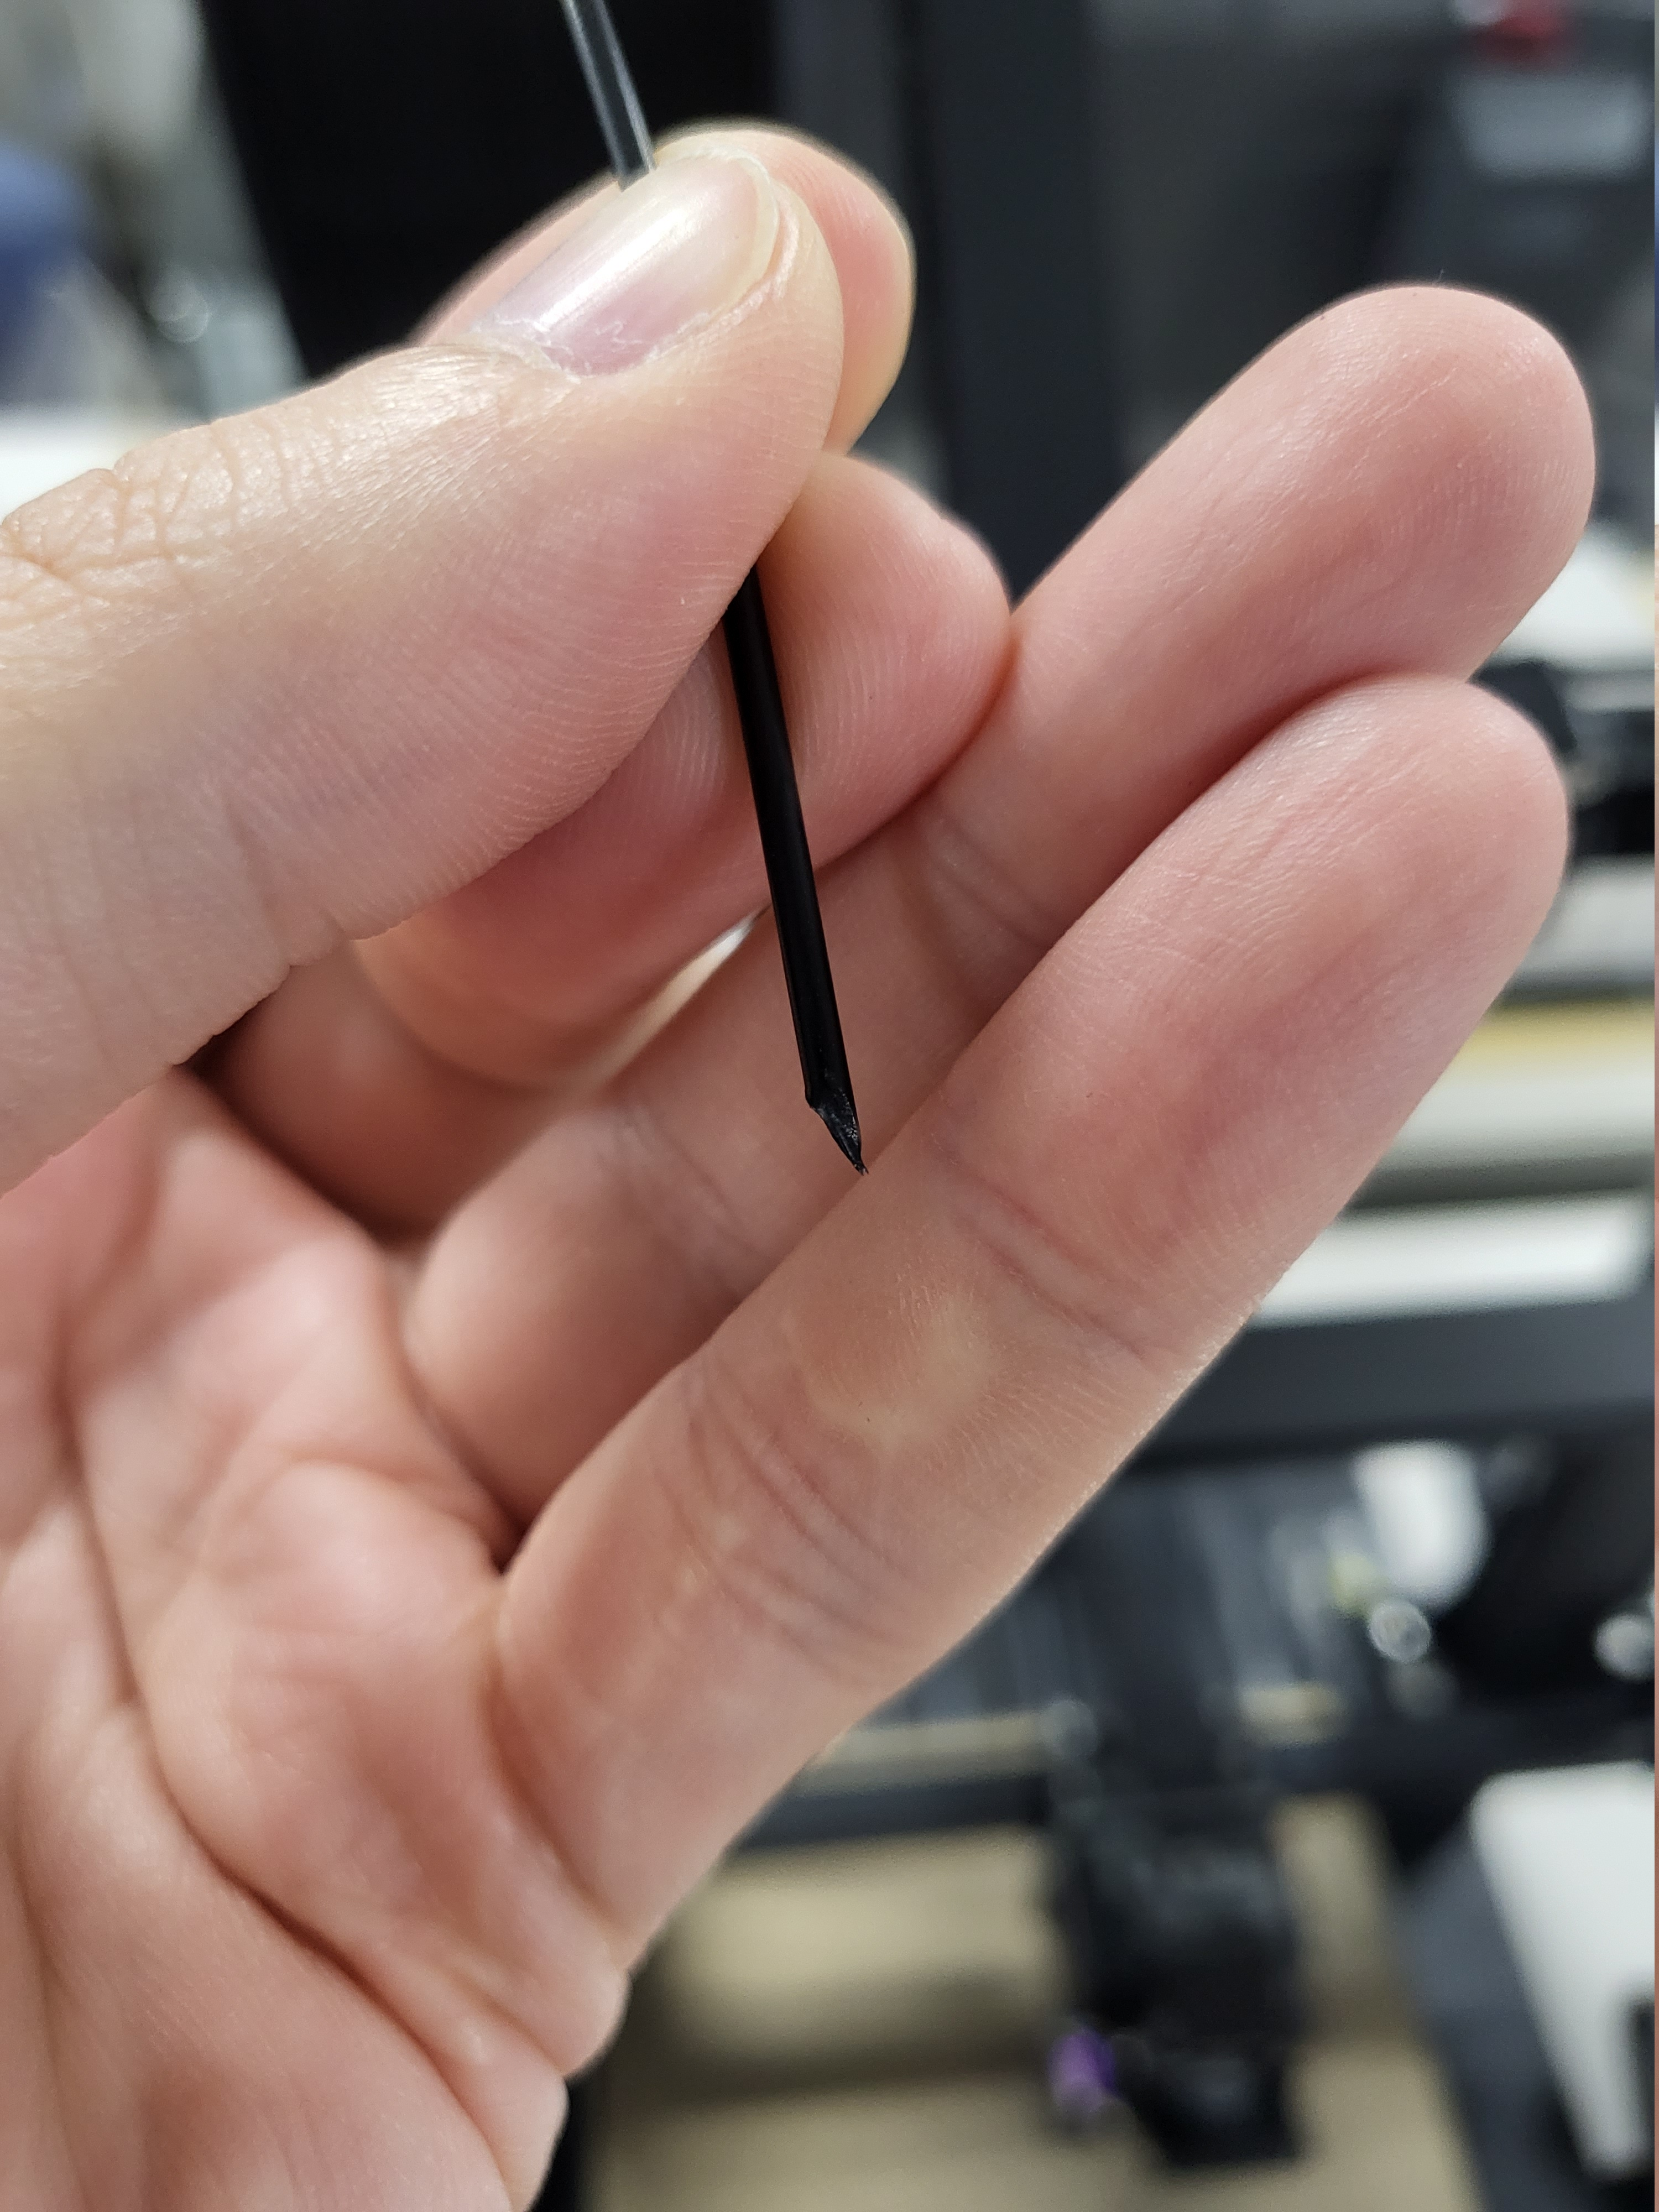
\includegraphics[width=0.4\textwidth]{img/ender/7.jpg} 
    \caption{When inserting a new fillament, it is a good idea to cut the tip in a wegded shap, making it easier to be gripped by the printing head.}
    \label{fig:ender7}
\end{figure}

\begin{figure}[H]
    \centering 
    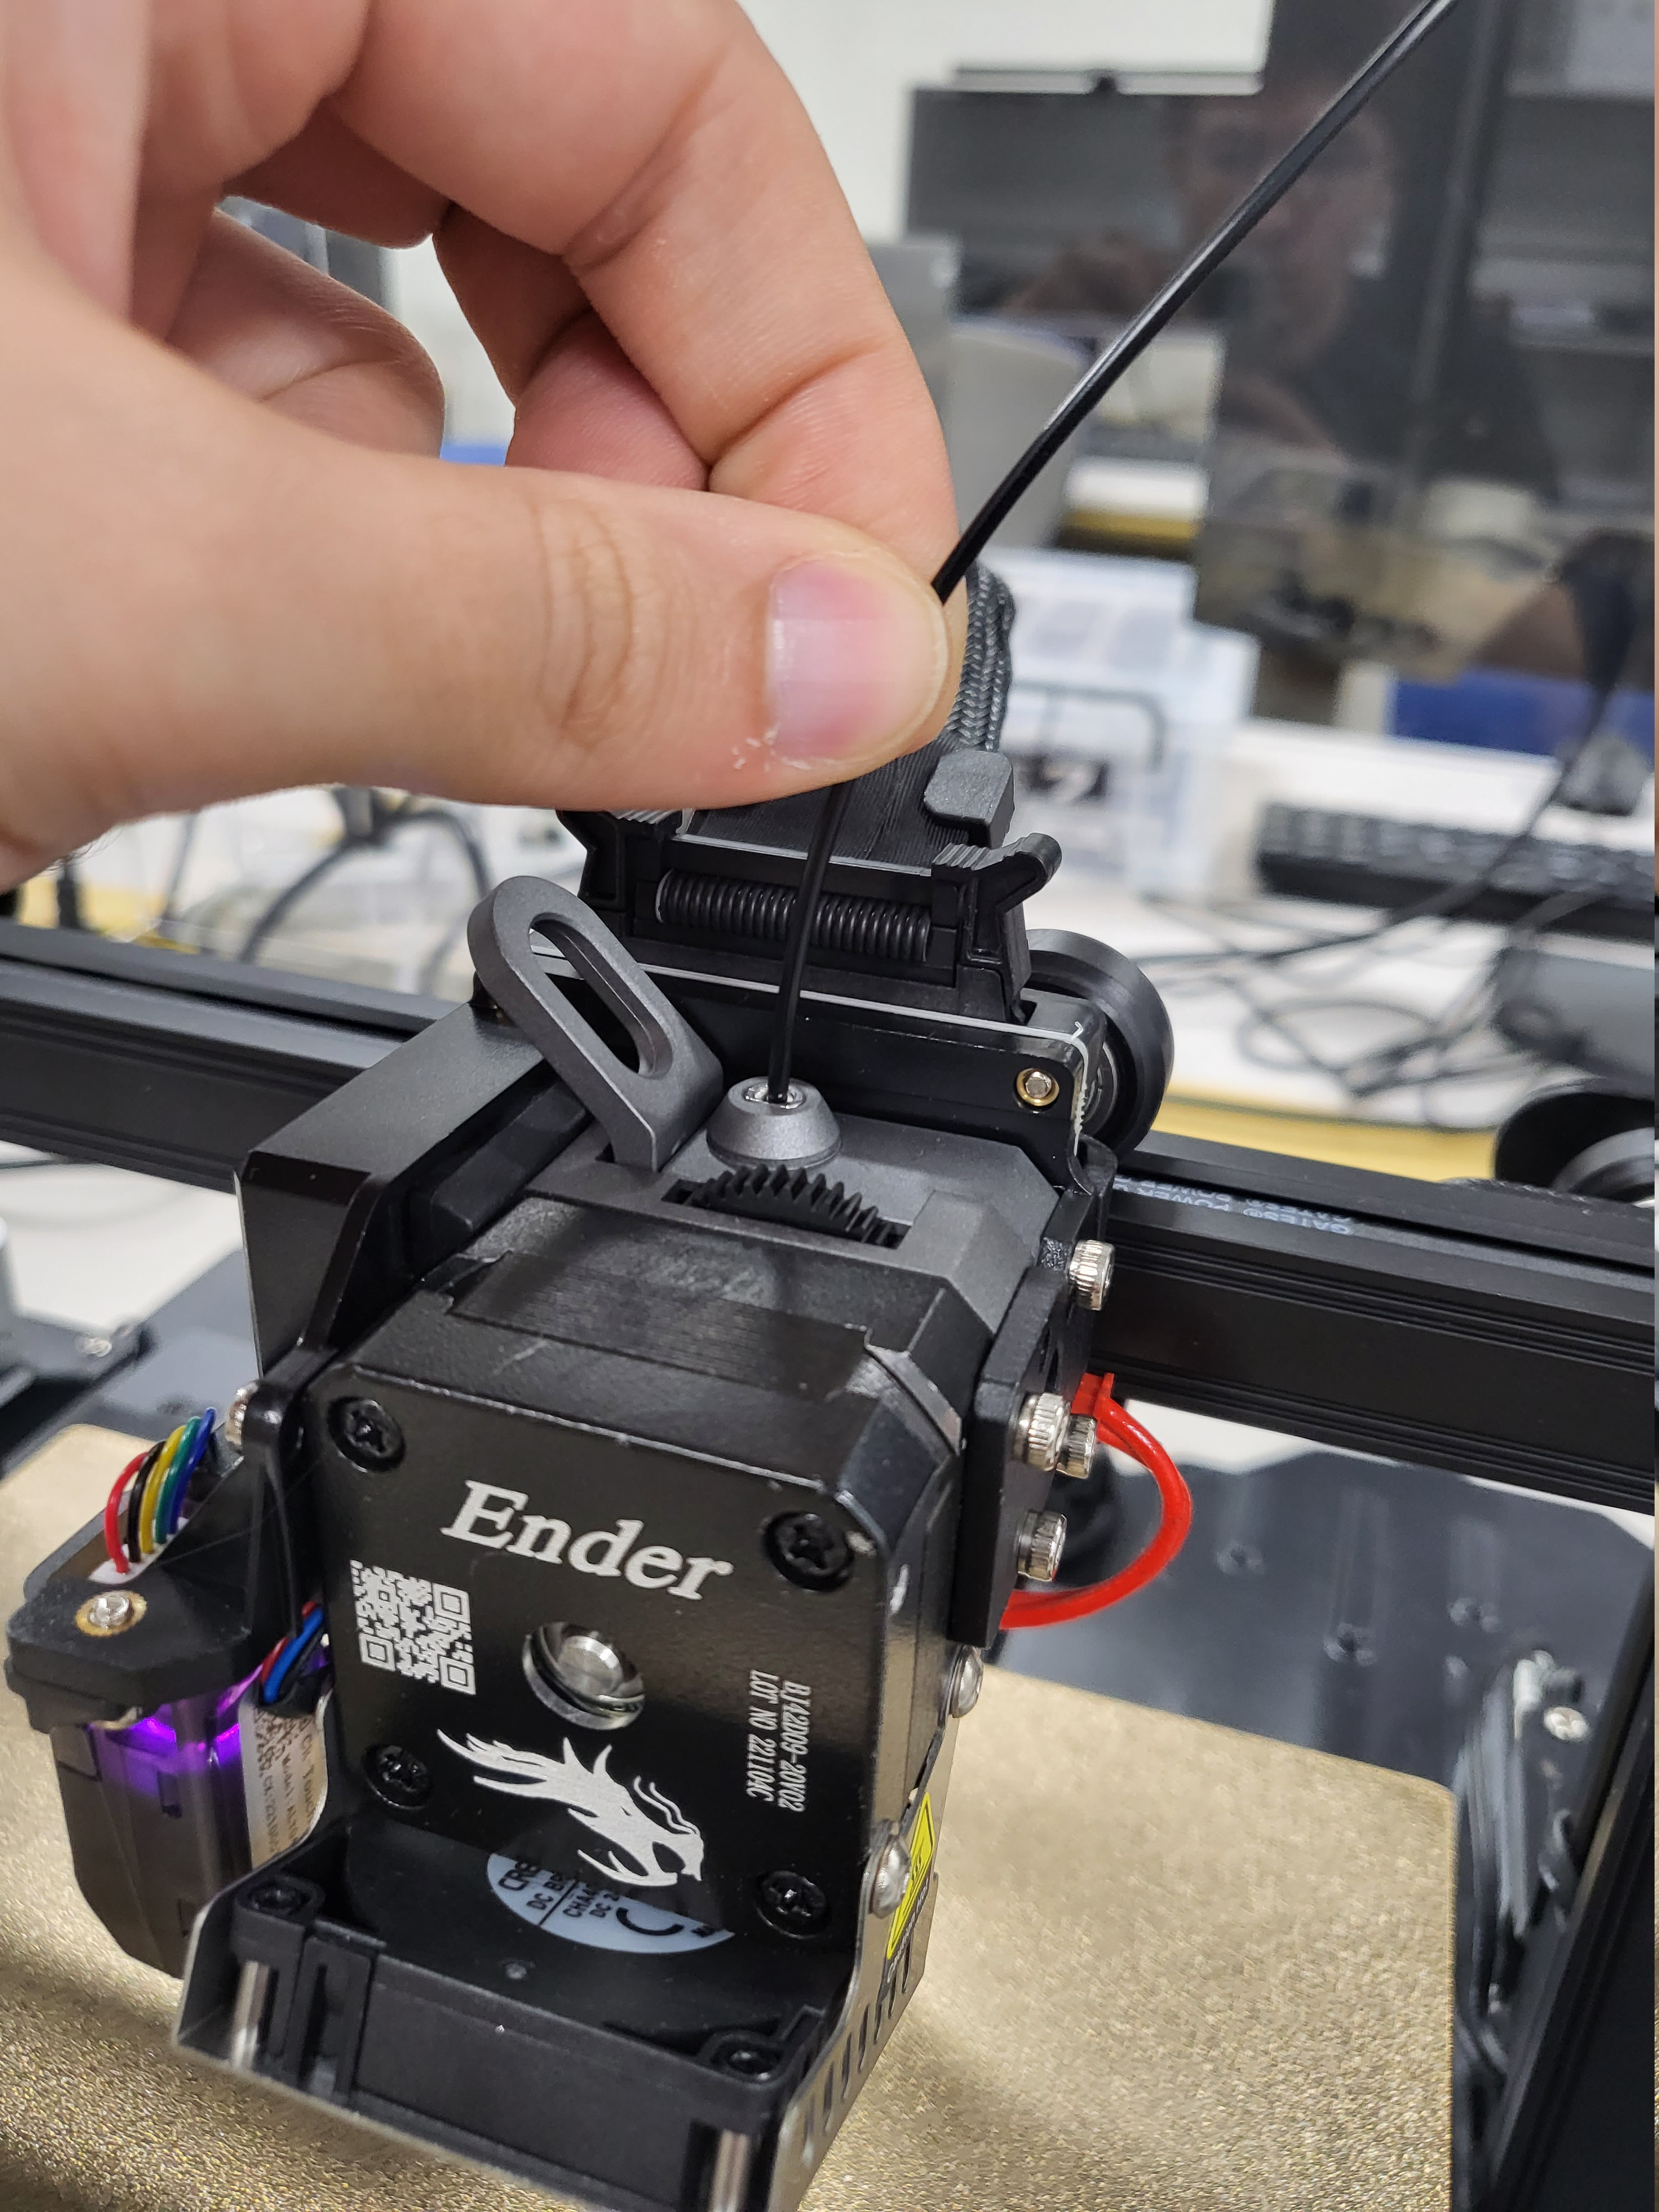
\includegraphics[width=0.4\textwidth]{img/ender/8.jpg} 
    \caption{The fillament being inserted in the printing head. Note that the nozzle should already be heated when doing so.}
    \label{fig:ender8}
\end{figure}


\subsection{Practice: Printing Benchy}
From that point we are ready to start printing our Benchy model.
The sliced model can be loaded on the printer's SD card, inserted in the machine and the printing can start.
\label{sec:org72afed1}
\begin{figure}[H]
    \centering 
    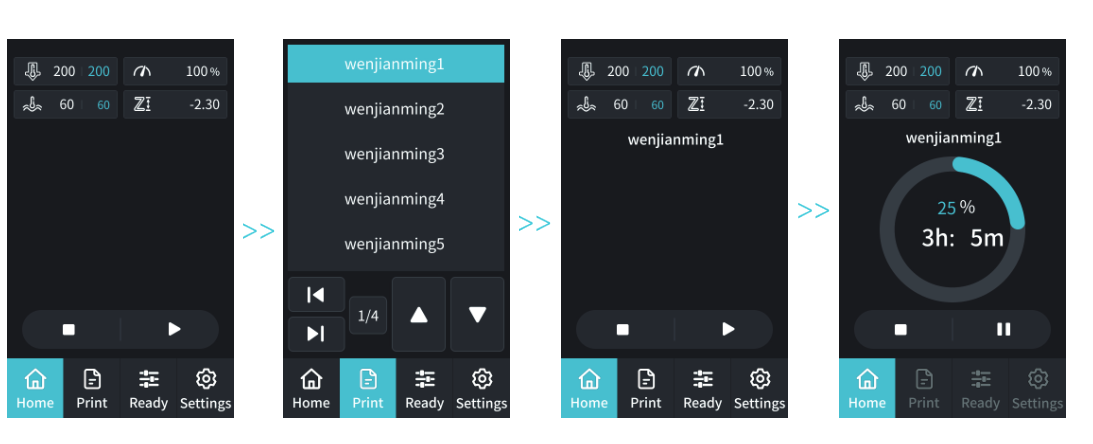
\includegraphics[width=0.8\textwidth]{img/ender/8a.png} 
    \caption{With the SD card inserted in the printer, it is possible to select the model, start heating the system and eventually the printing of the part will start.\\
    \textit{Source:} \href{https://img.staticdj.com/8f39f619af6bf34e5afb36ddbf2a0229.pdf?spm=..page\_1995605.download\_support\_1.1\&spm\_prev=..product\_5e45abfb-4541-4c92-ba93-cfba9a1e3ea4.nav\_link\_store\_1.1}{the reference manual}}
    \label{fig:ender8a}
\end{figure}

\begin{figure}[H]
    \centering 
    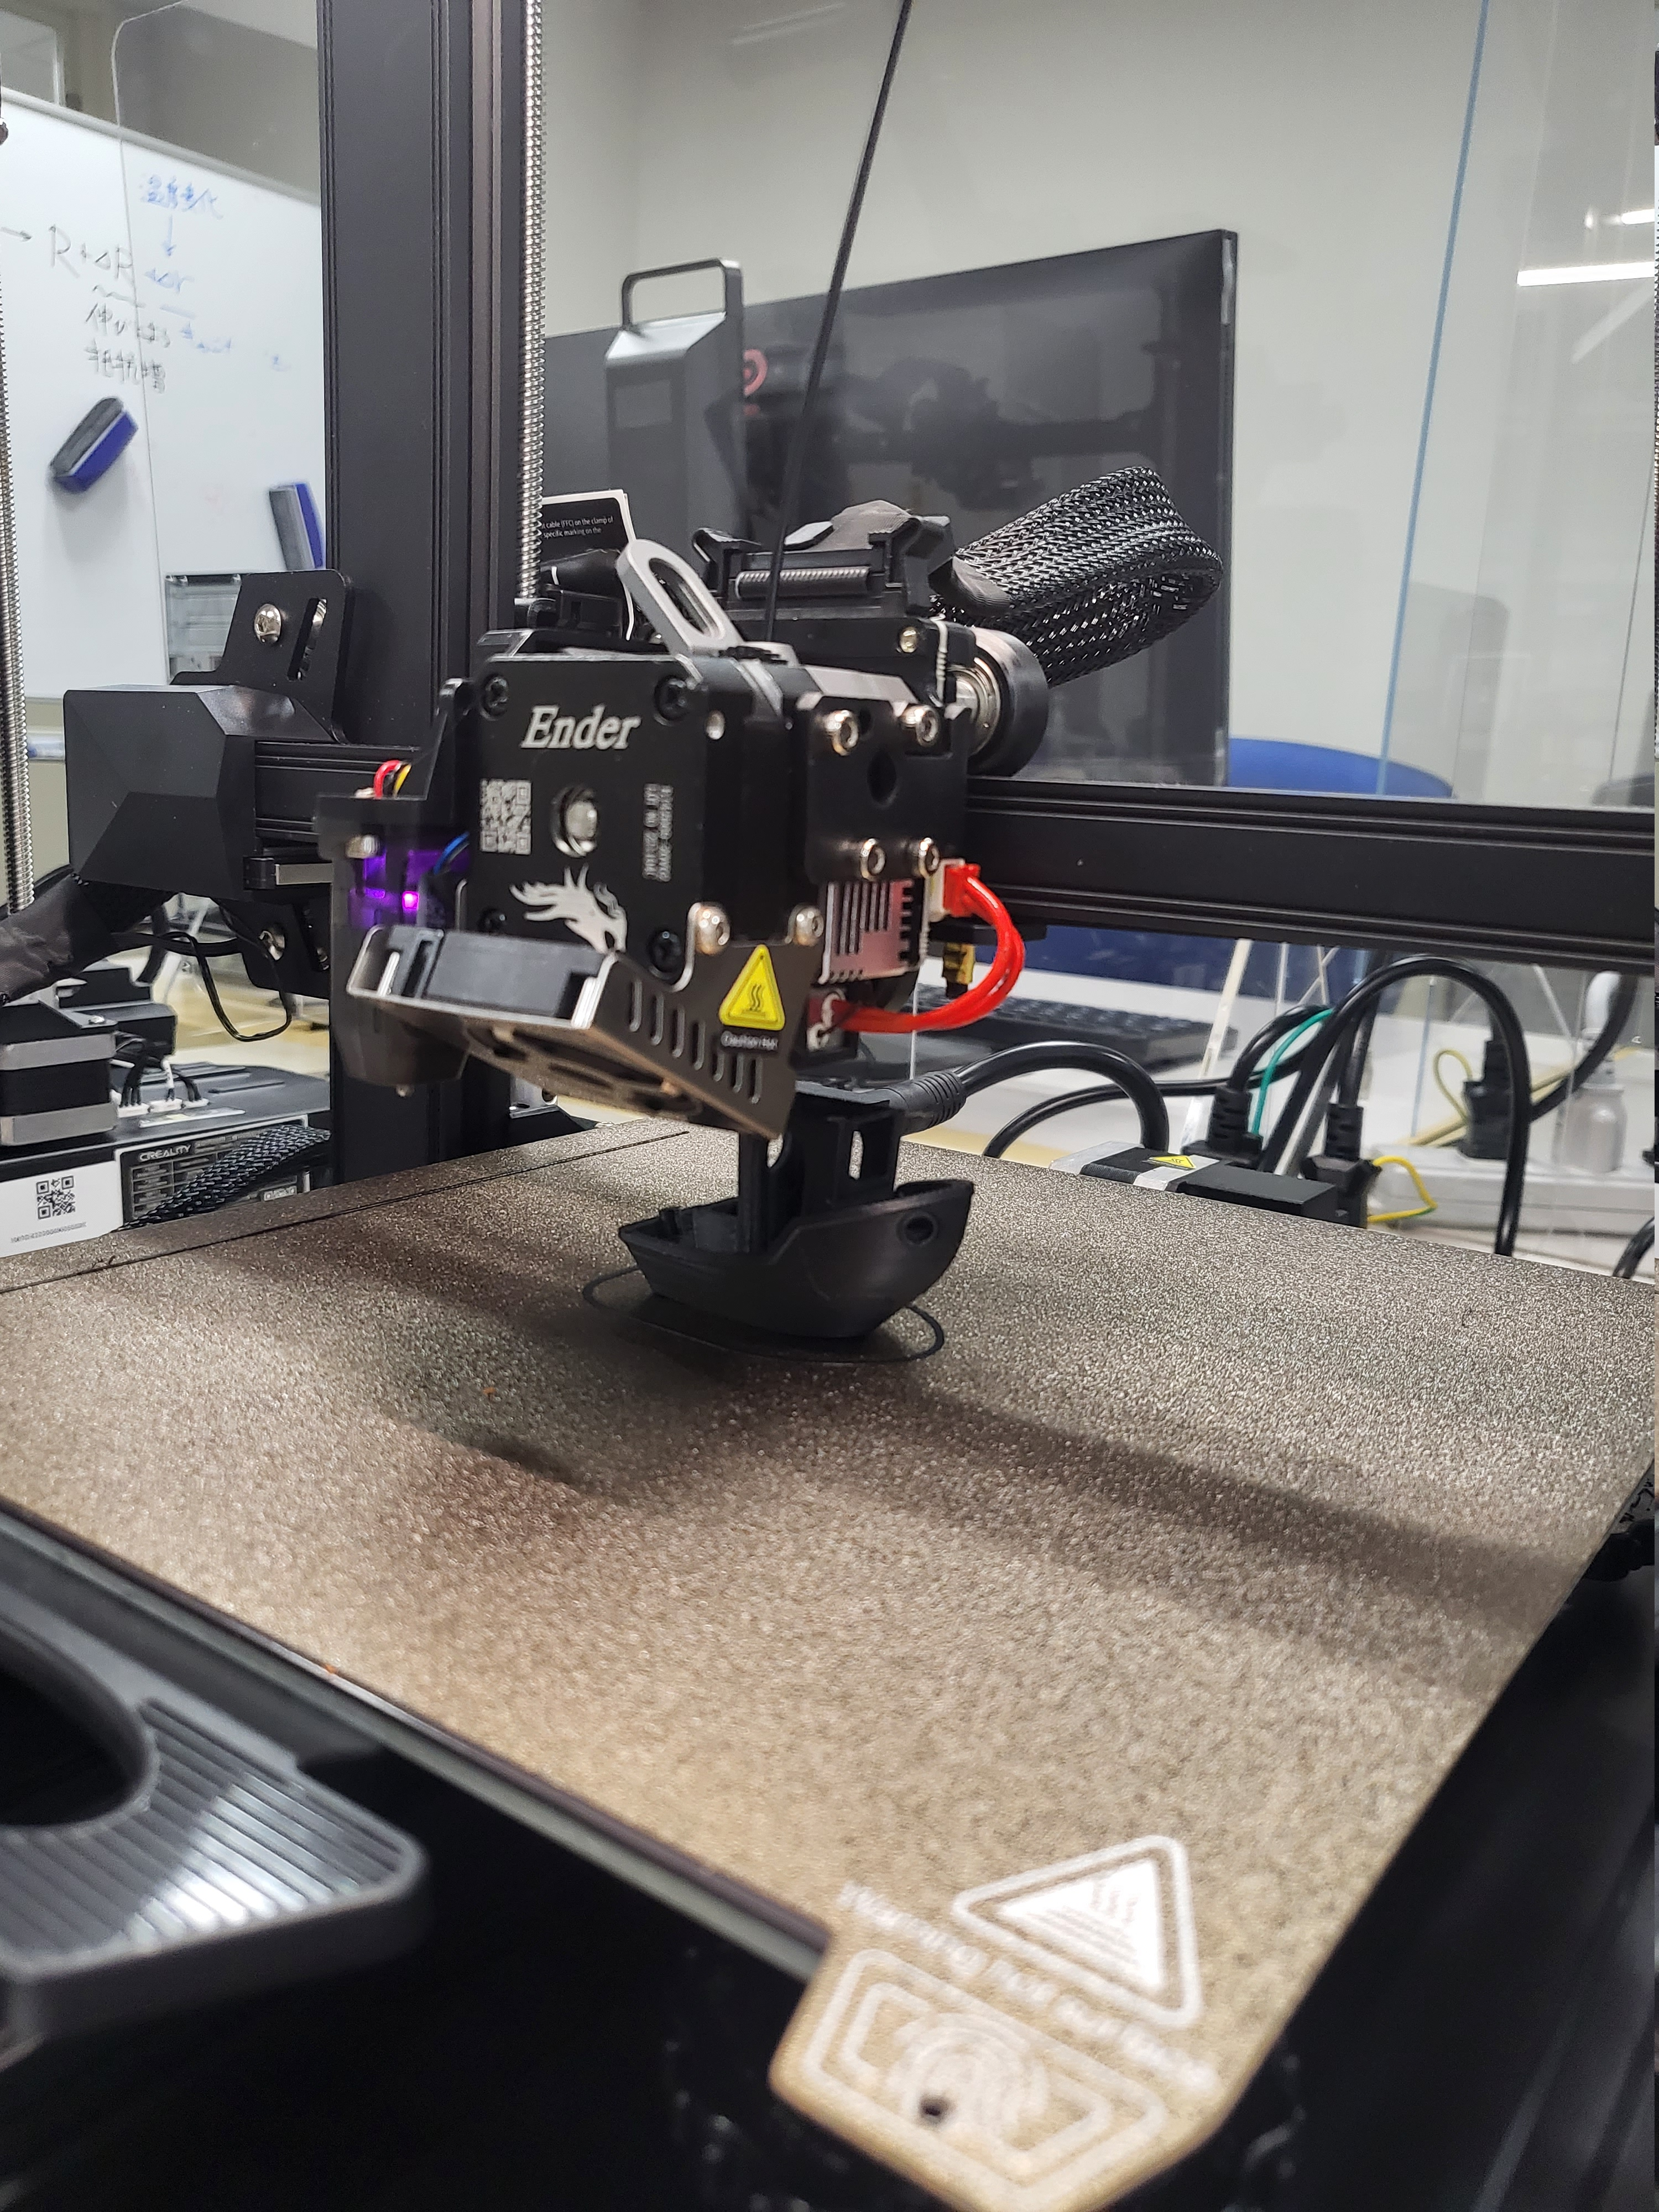
\includegraphics[width=0.6\textwidth]{img/ender/9.jpg} 
    \caption{Benchy being printed.}
    \label{fig:ender9}
\end{figure}

\begin{figure}[H]
    \centering 
    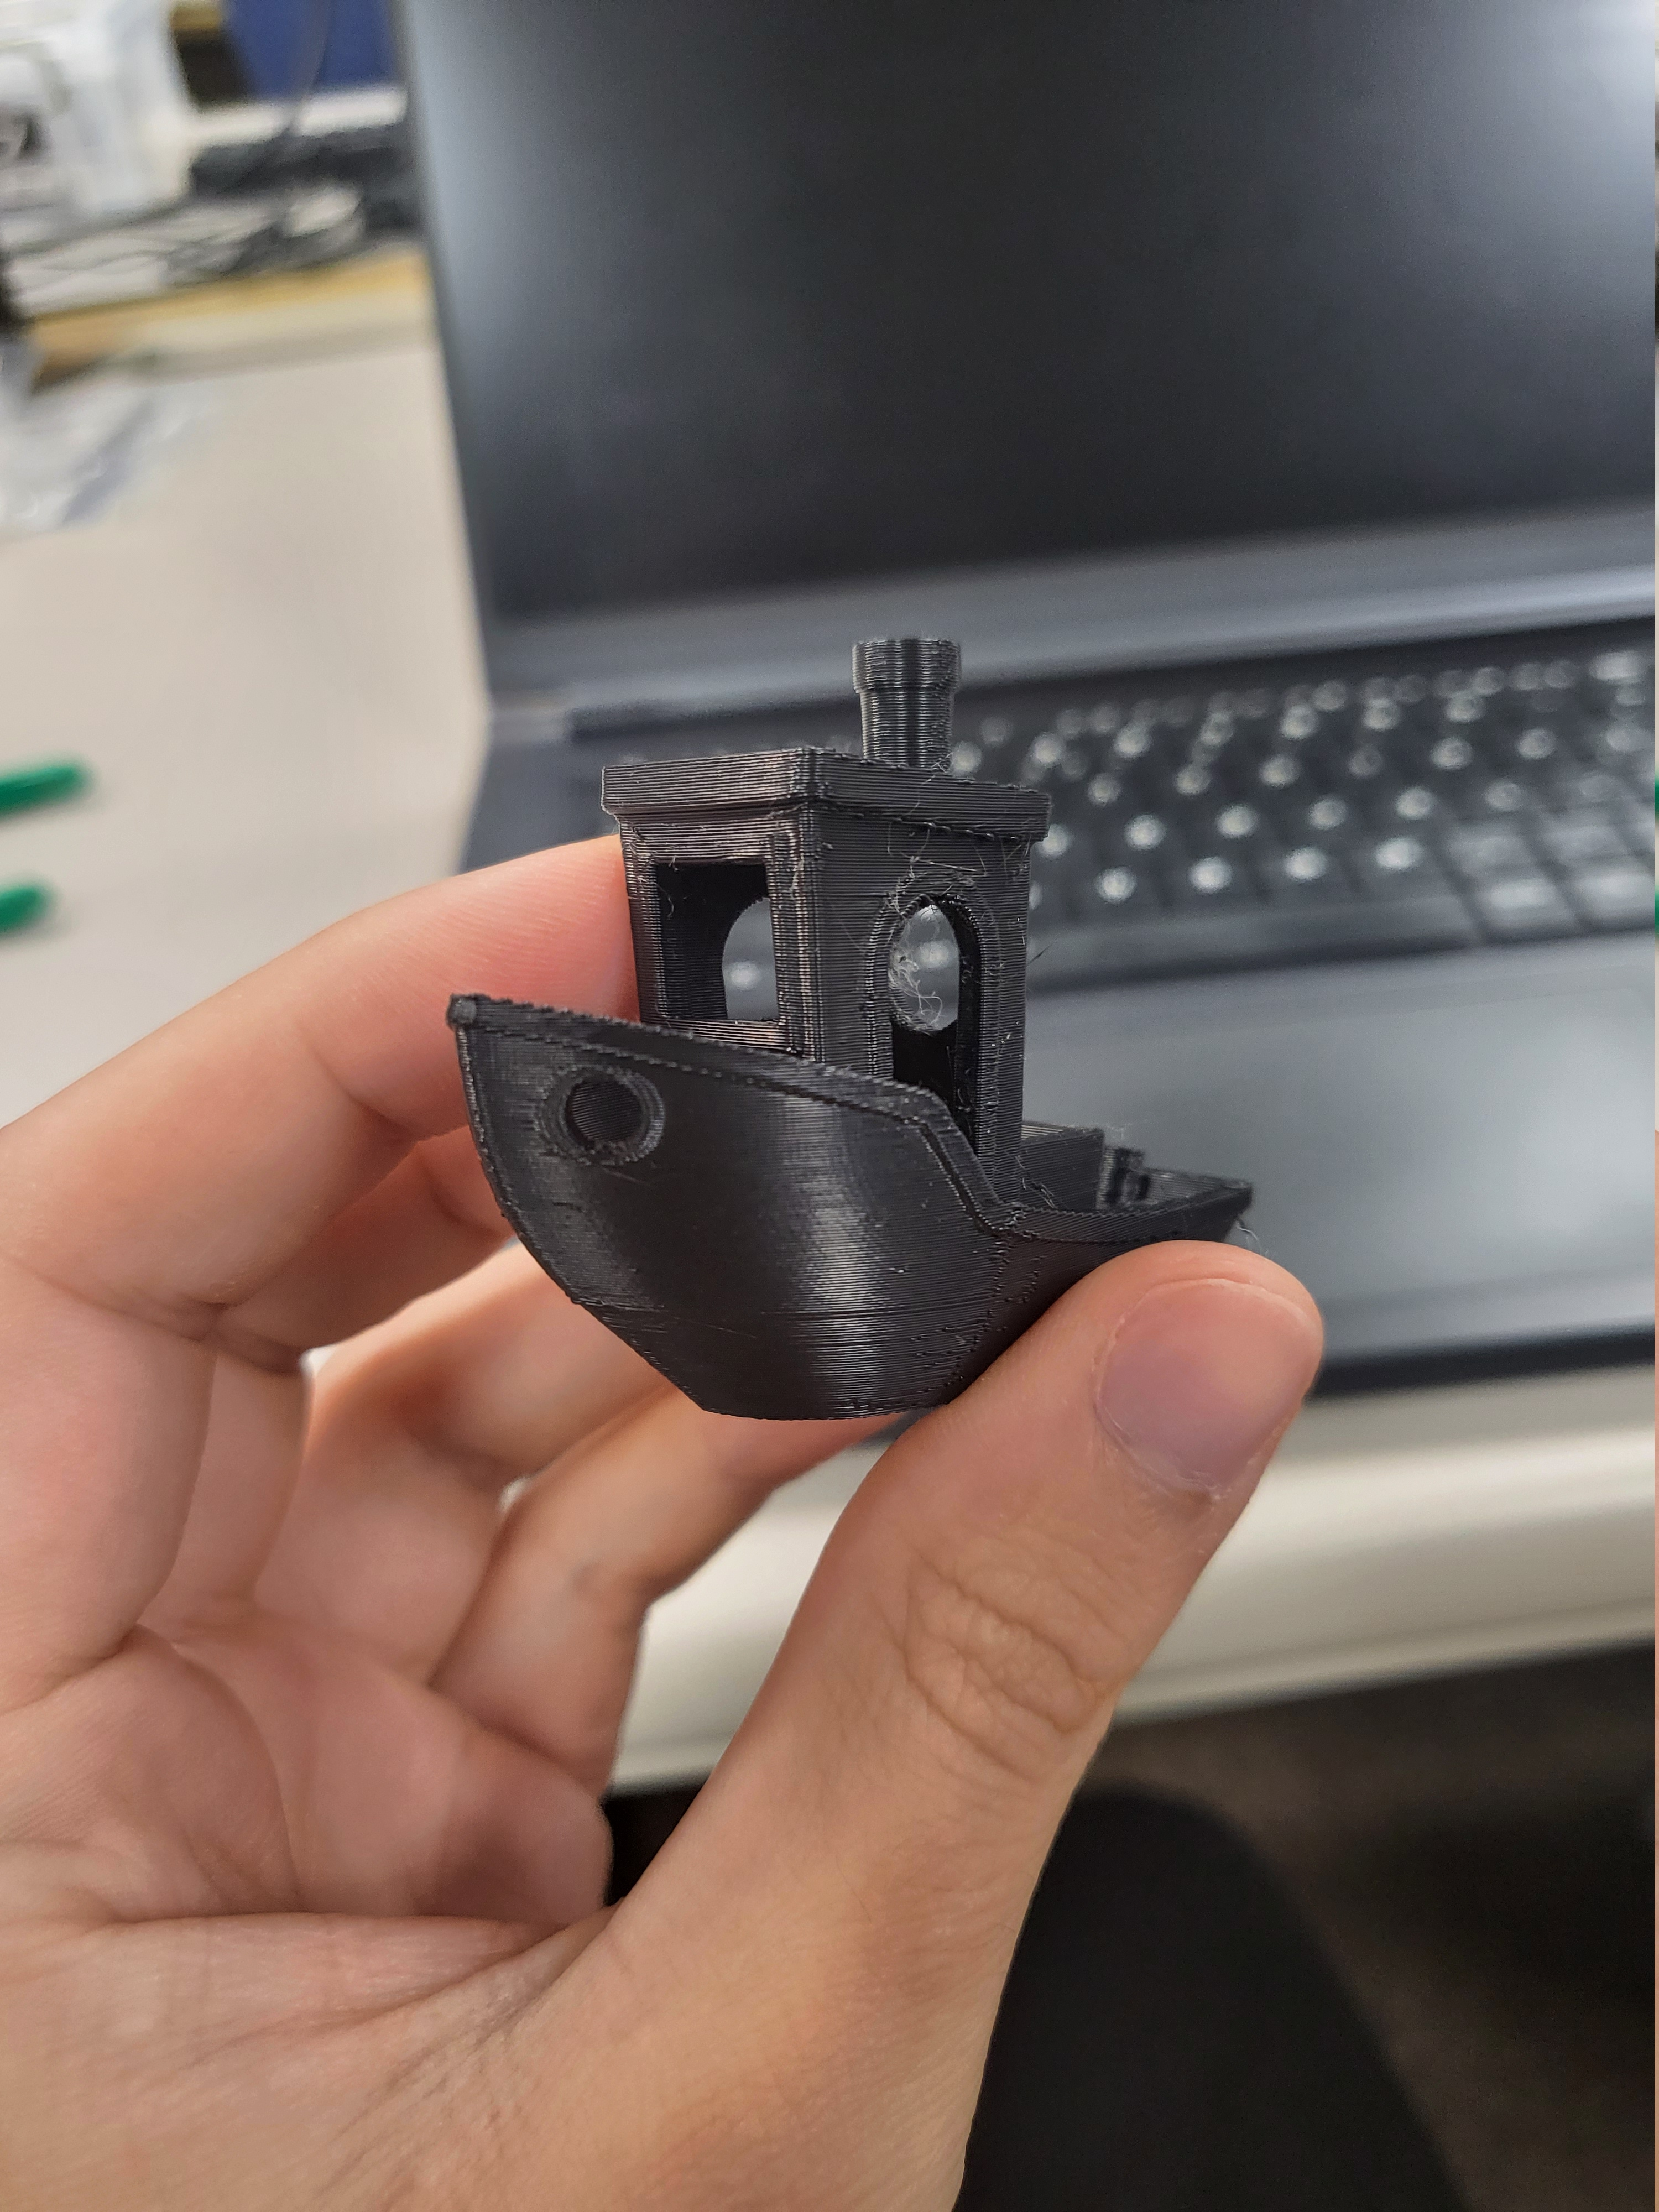
\includegraphics[width=0.6\textwidth]{img/ender/10.jpg} 
    \caption{Result! We can see some printing defects that will eventually require fine adjustment of the printer's settings and temperatures.}
    \label{fig:ender10}
\end{figure}


% ==============================================================================
% WIP
%\pagebreak
%\section{Troubleshooting}
%\label{sec:orgdabc8f0}


% ==============================================================================
\pagebreak
\section{Maintenance advice}
\label{sec:org4b6b33d}

\subsection{Moisture}
\label{sec:org8102bbe}
3D printing filament spools typically react poorly to moisture exposure.
If a spool is not to be used for an extended period of time, it should be removed from the printer,
put back in it's box, and kept close, ideally with a silicate get bag inside.
\end{document}
% instructions.tex document ends here